%%%%%%%%%%%%%%%%%%%%%%%%%%%%%%%%%%%%%%%%%%%%%%%%%%%%%%%%%%%%%%%
%
% Welcome to Overleaf --- just edit your LaTeX on the left,
% and we'll compile it for you on the right. If you open the
% 'Share' menu, you can invite other users to edit at the same
% time. See www.overleaf.com/learn for more info. Enjoy!
%
%%%%%%%%%%%%%%%%%%%%%%%%%%%%%%%%%%%%%%%%%%%%%%%%%%%%%%%%%%%%%%%
\documentclass[a4paper,UKenglish,cleveref, autoref, thm-restate]{lipics-v2021}
%\usepackage{semantic}
%\usepackage[margin=0.6in]{geometry}
%% Some recommended packages.
\usepackage{booktabs}   %% For formal tables:
                        %% http://ctan.org/pkg/booktabs
\usepackage{subcaption} %% For complex figures with subfigures/subcaptions
                        %% http://ctan.org/pkg/subcaption
\usepackage{bussproofs}
\usepackage[cal=boondoxo]{mathalfa}
\DeclareMathAlphabet{\mathpzc}{OT1}{pzc}{m}{it}
\usepackage{amsmath}
%\newtheorem{theorem}{Theorem}[section]
%\newtheorem{observation}[theorem]{Observation}
\usepackage{color}
\usepackage{xspace}
\newcommand{\comm}[3][\color{red}]{{#1{[{#2}: {#3}]}}}
%\newcommand{\comm}[3][\color{red}]{}
%\newcommand{\mwh}[1]{\comm[\color{blue}]{Mike}{#1}}

%\input{prooftree}

\newcommand{\ignore}[1]{{}}
\newcommand{\CTLK}{\textbf{CTLK}\xspace}
\newcommand{\TransK}{\textbf{TransK}\xspace}
\newcommand{\IsaK}{\textbf{IsaK}\xspace}
\newcommand{\IsaKa}{\textbf{IsaK+}\xspace}
\def\mcirc{\mathord{\scalebox{1.5}[1]{\scalerel*{\circ}{\strut}}}}
\def\msquare{\mathord{\scalerel*{\Box}{gX}}}
%\newcommand{\K}{\ensuremath{\mathbb{K}}\xspace}
\newcommand{\core}{\textbf{CORE}\xspace}
%\newcommand{\syntax}{\textbf{SYNTAX}\xspace}
\newcommand{\syntaxConstr}{\textbf{Syntax}\xspace}
\newcommand{\tokenConstr}{\textbf{Token}\xspace}
\newcommand{\subsortConstr}{\textbf{Subsort}\xspace}
\newcommand{\listSyntaxConstr}{\textbf{ListSyntax}\xspace}
\newcommand{\terminalConstr}{\textbf{Terminal}\xspace}
\newcommand{\nonterminalConstr}{\textbf{NonTerminal}\xspace}
\newcommand{\getStackType}{\texttt{getStackType}\xspace}
\newcommand{\gtop}{\texttt{top}\xspace}
\newcommand{\pick}{\texttt{pick}\xspace}
\newcommand{\match}{\texttt{match}\xspace}
\newcommand{\subst}{\texttt{subst}\xspace}
%\newcommand{\norm}{\texttt{norm}\xspace}
\newcommand{\typed}{\texttt{typed}\xspace}
\newcommand{\nelist}{\texttt{nelist}\xspace}
\newcommand{\genList}{\texttt{list}\xspace}
\newcommand{\genSet}{\texttt{set}\xspace}
\newcommand{\genLists}{\texttt{lists}\xspace}
\newcommand{\astring}{\texttt{string}\xspace}
\newcommand{\regex}{\texttt{regex}\xspace}
\newcommand{\theSymbol}{\texttt{symbol}\xspace}
\newcommand{\sortId}{\texttt{sortId}\xspace}
\newcommand{\cellId}{\texttt{cellId}\xspace}
\newcommand{\metaId}{\texttt{metaId}\xspace}
\newcommand{\labelId}{\texttt{labelId}\xspace}
\newcommand{\ir}{\textbf{IR}\xspace}
\newcommand{\cool}{\texttt{cool}\xspace}
\newcommand{\forname}{\constant{forname}\;}
\newcommand{\kif}{\constant{if}\;}
\newcommand{\kthen}{\constant{then}\;}
\newcommand{\kelse}{\constant{else}\;}
\newcommand{\kskip}{\constant{skip}\;}
\newcommand{\loopin}{\constant{in}\;}
\newcommand{\heat}{\texttt{heat}\xspace}
\newcommand{\kCell}{\texttt{kCell}\xspace}
\newcommand{\KResult}{\texttt{KResult}\xspace}
\newcommand{\kSyntax}{\texttt{kSyntax}\xspace}
\newcommand{\syntaxDef}[3]{\rulebox{%
\syntaxKeyword$#1\mathrel{::=}{#2}$ \ifthenelse{\equal{#3}{}}{}{[#3]}%
}%
}
\newcommand{\kvariable}[2]{\variable{#1}:\variable{#2}}
\newcommand{\kRule}{\texttt{kRule}\xspace}
\newcommand{\kRules}{\texttt{kRules}\xspace}
\newcommand{\irKRule}{\texttt{irKRule}\xspace}
\newcommand{\irKRules}{\texttt{irKRules}\xspace}
\newcommand{\kFile}{\texttt{kFile}\xspace}
\makeatletter
\newcommand{\shorteq}{%
  \settowidth{\@tempdima}{-}% Width of hyphen
  \resizebox{\@tempdima}{\height}{=}%
}
\makeatother


\newcommand{\RuleLabel}{\textit{RuleLabel}\xspace}
\newcommand{\RuleLabels}{\textit{RuleLabels}\xspace}
\newcommand{\QuestionKey}{\mathbf{?}\xspace}
\newcommand{\StarKey}{\mathbf{*}\xspace}
\newcommand{\Stream}{\textbf{Stream}\xspace}
\newcommand{\stdWord}{\texttt{std}\xspace}
\newcommand{\Multiplicity}{\textbf{Multiplicity}\xspace}
\newcommand{\keyWord}{\texttt{key}\xspace}
\newcommand{\feature}{\texttt{feature}\xspace}
\newcommand{\Context}{\textbf{Context}\xspace}
\newcommand{\Fun}{\textbf{Fun}\xspace}
\newcommand{\FunRule}{\textbf{FunRule}\xspace}
\newcommand{\FunRules}{\textbf{FunRules}\xspace}
\newcommand{\Macro}{\textbf{Macro}\xspace}
\newcommand{\MacroRule}{\textbf{MacroRule}\xspace}
\newcommand{\MacroRules}{\textbf{MacroRules}\xspace}
\newcommand{\Anywhere}{\textbf{Anywhere}\xspace}
\newcommand{\AnywhereRule}{\textbf{AnywhereRule}\xspace}
\newcommand{\AnywhereRules}{\textbf{AnywhereRules}\xspace}
\newcommand{\KNormal}{\textbf{KNormal}\xspace}
\newcommand{\KNormalRule}{\textbf{KNormalRule}\xspace}
\newcommand{\KNormalRules}{\textbf{KNormalRules}\xspace}
\newcommand{\BagNormal}{\textbf{BagNormal}\xspace}
\newcommand{\BagNormalRule}{\textbf{BagNormalRule}\xspace}
\newcommand{\BagNormalRules}{\textbf{BagNormalRules}\xspace}
\newcommand{\synAttr}{\texttt{synAttrib}\xspace}
\newcommand{\ruleAttr}{\texttt{ruleAttrib}\xspace}
\newcommand{\synAttrs}{\texttt{synAttribs}\xspace}
\newcommand{\ruleAttrs}{\texttt{ruleAttribs}\xspace}
\newcommand{\Strict}{\texttt{Strict}\xspace}
\newcommand{\productions}{\texttt{productions}\xspace}
\newcommand*{\Leadsto}{\ensuremath{\leadsto}\xspace}
\newcommand{\bigK}{\texttt{bigK}\xspace}
\newcommand{\bigKBag}{\texttt{bigKBag}\xspace}
\newcommand{\constType}{\texttt{const}\xspace}
\newcommand{\kLabel}{\texttt{kLabel}\xspace}
\newcommand{\kLabels}{\texttt{kLabels}\xspace}
\newcommand{\irPat}{\texttt{irFunPat}\xspace}
\newcommand{\irFunApp}{\texttt{irFunApp}\xspace}
\newcommand{\funApp}{\texttt{funApp}\xspace}
\newcommand{\irKLabel}{\texttt{irKLabel}\xspace}
\newcommand{\irKLabels}{\texttt{irKLabels}\xspace}
\newcommand{\kItem}{\texttt{kItem}\xspace}
\newcommand{\kItems}{\texttt{kItems}\xspace}
\newcommand{\irKItem}{\texttt{irKItem}\xspace}
\newcommand{\irKItems}{\texttt{irKItems}\xspace}
\newcommand{\irBigKBag}{\texttt{irBigKBag}\xspace}
\newcommand{\irBigKBagLabel}{\texttt{irBigKBagLabel}\xspace}
\newcommand{\kList}{\texttt{kList}\xspace}
\newcommand{\kLists}{\texttt{kLists}\xspace}
\newcommand{\irKListElem}{\texttt{irKListElem}\xspace}
\newcommand{\irKList}{(\texttt{irKListElem\;\genList})\xspace}
\newcommand{\irKLists}{(\texttt{irKListElem\;\genLists})\xspace}
\newcommand{\ak}{\texttt{k}\xspace}
\newcommand{\aks}{\texttt{ks}\xspace}
\newcommand{\irKElem}{\texttt{irKElem}\xspace}
\newcommand{\irK}{(\texttt{irKElem\;\genList})\xspace}
\newcommand{\irKs}{(\texttt{irKElem\;\genLists})\xspace}
\newcommand{\alist}{\texttt{aList}\xspace}
\newcommand{\alists}{\texttt{aLists}\xspace}
\newcommand{\irListElem}{\texttt{irListElem}\xspace}
\newcommand{\irList}{(\texttt{irListElem\xspace\genList})\xspace}
\newcommand{\irLists}{(\texttt{irListElem\xspace\genLists})\xspace}
\newcommand{\set}{\texttt{set}\xspace}
\newcommand{\sets}{\texttt{sets}\xspace}
\newcommand{\irSetElem}{\texttt{irSetElem}\xspace}
\newcommand{\irSet}{(\texttt{irSetElem\;\genList})\xspace}
\newcommand{\irSets}{(\texttt{irSetElem\;\genLists})\xspace}
\newcommand{\map}{\texttt{map}\xspace}
\newcommand{\maps}{\texttt{maps}\xspace}
\newcommand{\irMapElem}{\texttt{irMapElem}\xspace}
\newcommand{\irMap}{(\texttt{irMapElem\;\genList})\xspace}
\newcommand{\irMaps}{(\texttt{irMapElem\;\genLists})\xspace}
\newcommand{\cell}{\texttt{cell}\xspace}
\newcommand{\cells}{\texttt{cells}\xspace}
\newcommand{\bag}{\texttt{bag}\xspace}
\newcommand{\bags}{\texttt{bags}\xspace}
\newcommand{\irBagElem}{\texttt{irBagElem}\xspace}
\newcommand{\irBag}{(\texttt{irBagElem\;\genList})\xspace}
\newcommand{\irBags}{(\texttt{irBagElem\;\genLists})\xspace}
\newcommand{\rewrite}{\texttt{rewrite}\xspace}
\newcommand{\rewriteConstr}{\textbf{Rewrite}\xspace}
\newcommand{\rewriteConstrs}{\textbf{Rewrites}\xspace}
\newcommand{\program}{\texttt{program}\xspace}
\newcommand{\kompile}{\textbf{\textit{kompile}}\xspace}
\newcommand{\krun}{\textbf{\textit{krun}}\xspace}
\newcommand{\ksearch}{\textbf{\textit{ksearch}}\xspace}
\newcommand{\ktheory}{\ensuremath{\mathbb{K}}\texttt{\_theory}\xspace}

\newcommand{\genKLabel}{\texttt{genKLabel}\xspace}
\newcommand{\regexPar}{\texttt{regexPar}\xspace}

\newcommand{\kLabelSort}{\texttt{KLabel}\xspace}
\newcommand{\kItemSort}{\texttt{KItem}\xspace}
\newcommand{\kListSort}{\texttt{KList}\xspace}
\newcommand{\kSort}{\texttt{K}\xspace}
\newcommand{\listSort}{\texttt{List}\xspace}
\newcommand{\setSort}{\texttt{Set}\xspace}
\newcommand{\mapSort}{\texttt{Map}\xspace}
\newcommand{\bagSort}{\texttt{Bag}\xspace}

\newcommand{\topSort}{\texttt{topSort}\xspace}
\newcommand{\KItemIR}{\textbf{KItemIR}\xspace}
\newcommand{\IdKItemIR}{\textbf{IdKItemIR}\xspace}
\newcommand{\HOLEIR}{\textbf{HOLEIR}\xspace}
\newcommand{\KListElemIR}{\textbf{KListElemIR}\xspace}
\newcommand{\KListIdIR}{\textbf{KListIdIR}\xspace}
\newcommand{\strict}{\texttt{strict}\xspace}
\newcommand{\seqstrict}{\texttt{seqstrict}\xspace}
%\newcommand{\function}{\texttt{function}\xspace}
\newcommand{\klabelAttr}{\textbf{Klabel}\xspace}
\newcommand{\macroAttr}{\texttt{macro}\xspace}
\newcommand{\anywhereAttr}{\texttt{anywhere}\xspace}
\newcommand{\owiseAttr}{\textbf{Owise}\xspace}
\newcommand{\Transition}{\texttt{Transition}\xspace}
\newcommand{\transition}{\texttt{transition}\xspace}
\newcommand{\add}{\texttt{add}\xspace}
\newcommand{\hasFunTerm}{\texttt{hasFunTerm}\xspace}
\newcommand{\funMatch}{\texttt{funMatch}\xspace}
\newcommand{\kNormMatch}{\texttt{kNormMatch}\xspace}
\newcommand{\bagNormMatch}{\texttt{bagNormMatch}\xspace}
\newcommand{\anywhereMatch}{\texttt{anywhereMatch}\xspace}
\newcommand{\macroMatch}{\texttt{macroMatch}\xspace}
\newcommand{\sortAdjust}{\texttt{sortAdjust}\xspace}
\newcommand{\validMacroRules}{\texttt{validMacroRules}\xspace}
\newcommand{\getKLabel}{\texttt{getKLabel}\xspace}
\newcommand{\isFunLabel}{\texttt{isFunLabel}\xspace}
\newcommand{\cut}{\texttt{split}\xspace}
\newcommand{\compile}{\texttt{compile}\xspace}
\newcommand{\sortOf}{\texttt{sortOf}\xspace}
\newcommand{\argSortsOf}{\texttt{argSortsOf}\xspace}
\newcommand{\smallestSort}{\texttt{smallestSort}\xspace}
%\newcommand{\send}[3]{\textsf{!}[#1|#2]\to#3}

\newcommand{\letin}[3]{{\ensuremath{\textsf{let}\;{#1}={#2}\;\textsf{in}\;{#3}}}}
%[|(#2,#3)|#4|]#5
%% \newcommand{\bigparallels}[5]{{\ensuremath{
%% \begin{array}[t]{l}
%% #1\\
%%  |\![\!\{#2.#3|#4\}\!]\!|\\
%% #5
%% \end{array}}}}
\newcommand{\bigparallels}[5]{{\ensuremath{#1 |\![\!\{#2.#3|#4\}\!]\!|#5}}}
\newcommand{\seque}[2]{#1;#2}
\newcommand{\extchoices}[2]{#1\Box#2}
%\newcommand{\intchoices}[2]{#1|\sim|#2}
\newcommand{\intchoices}[2]{#1\sqcap#2}
\newcommand{\hiding}[4]{#1\setminus\{#2.#3|#4\}}
\newcommand{\rename}[6]{#1\;\ensuremath{[\![\!\{((#2.#3),(#4.#5))|#6\}\!]\!]}}
\newcommand{\WT}[1]{\textsf{Wf}(\textsf{#1})}

\newcommand{\LOGICAND}{{\textsf{Conjunction}}}
\newcommand{\LOGICOR}{{\textsf{Disjunction}}}
\newcommand{\LOGICNOT}{{\textsf{Negation}}}
\newcommand{\WELLTYPE}{{\textsf{Well-formed}}}
\newcommand{\EQUALITY}{{\textsf{Equality}}}
\newcommand{\WEAKENLOGICOR}{{\textsf{Strong-disjunction}}}
\newcommand{\WEAKENLOGICNOT}{{\textsf{Strong-negation}}}


\newcommand{\reglai}[3]{
    \prooftree
         #1
    \justifies  
         #2
    \thickness=0.05em
    \using
        #3
    \endprooftree}

\newcommand{\reglaii}[4]{
    \prooftree
         #1\quad
         #2
    \justifies  
         #3
    \thickness=0.05em
    \using
        #4
    \endprooftree}

\newcommand{\sreglai}[3]{
    \prooftree
\begin{array}{c}
         #1
\end{array}
    \justifies  
         #2
    \thickness=0.05em
    \using
        #3
    \endprooftree}


\newcommand{\sreglaii}[4]{
    \prooftree
\begin{array}{c}
         #1\\
         #2
\end{array}
    \justifies  
         #3
    \thickness=0.05em
    \using
        #4
    \endprooftree}

\newcommand{\sreglaiii}[5]{
    \prooftree
\begin{array}{c}
         #1\\
         #2\\
	 #3
\end{array}
    \justifies  
         #4
    \thickness=0.05em
    \using
        #5
    \endprooftree}

\newcommand{\ssregla}[6]{
    \prooftree
\begin{array}{c}
         #1\\[-.7em]
         #2\\[-.7em]
	 #3\\[-.7em]
	 #4
\end{array}
    \justifies  
         #5
    \thickness=0.05em
    \using
        #6
    \endprooftree}


\newcommand{\reglaiii}[5]{
    \prooftree
         #1\quad
         #2\quad
         #3
    \justifies  
         #4
    \thickness=0.05em
    \using
        #5
    \endprooftree}

\newcommand{\reglaiv}[6]{
    \prooftree
         #1\quad
         #2\quad
         #3\quad
         #4
    \justifies  
         #5
    \thickness=0.05em
    \using
        #6
    \endprooftree}


\newcommand{\pist}{\ensuremath{\mathsf{Iris}}}

% Process terms
\newcommand{\chIn}[3]{\ensuremath{#1?(#2)\ \texttt{in}\ #3}}
\newcommand{\chOut}[2]{\ensuremath{#1![#2]}}
\newcommand{\palel}[2]{#1\ensuremath{|}\,#2}
\newcommand{\branch}{\ensuremath{\rhd}\,}
\newcommand{\select}{\ensuremath{\lhd}\,}
\newcommand{\new}[2]{\ensuremath{(\nu #1)#2}}
\newcommand{\inicioAss}[1]{\ensuremath{\texttt{begin}\ #1}}
\newcommand{\finAss}[1]{\ensuremath{\texttt{end}\ #1}}
\newcommand{\accept}[2]{\ensuremath{\texttt{accept}\ #1\ \texttt{in}\ #2}}
\newcommand{\request}[2]{\ensuremath{\texttt{request}\ #1\ \texttt{in}\ #2}}
\newcommand{\throw}[2]{\ensuremath{\texttt{throw}\ #1[#2]}}
\newcommand{\catch}[3]{\ensuremath{\texttt{catch}\ #1(#2)\ \texttt{in}\ #3}}
\newcommand{\defin}[2]{\ensuremath{\texttt{def}\ #1\ \texttt{in}\ #2}}
%\newcommand{\zero}{\ensuremath{\texttt{stop}}}
\newcommand{\callProc}[2]{\ensuremath{#1[#2]}}
\newcommand{\declProc}[3]{\ensuremath{#1[#2]=#3}}


% ATM example
\newcommand{\Atm}{\ensuremath{\textsf{ATM}}}
\newcommand{\Atmi}{\ensuremath{\textsf{ATM'}}}
\newcommand{\Atmii}{\ensuremath{\textsf{ATM''}}}
\newcommand{\Bank}{\ensuremath{\textsf{Bank}}}
\newcommand{\Client}{\ensuremath{\textsf{Client}}}
\newcommand{\Clienti}{\ensuremath{\textsf{Client'}}}
\newcommand{\Banki}{\ensuremath{\textsf{Bank'}}}
\newcommand{\atmDef}[1]{\ensuremath{\textsf{ATM}(#1)}}
\newcommand{\atmCall}[1]{\ensuremath{\textsf{ATM}[#1]}}
\newcommand{\bankDef}[1]{\ensuremath{\textsf{Bank}(#1)}}
\newcommand{\bankCall}[1]{\ensuremath{\textsf{Bank}[#1]}}
\newcommand{\clientDef}[1]{\ensuremath{\textsf{Client}(#1)}}
\newcommand{\clientCall}[1]{\ensuremath{\textsf{Client}[#1]}}

% Auction example
\newcommand{\Auctioneer}{\ensuremath{\textsf{Auctioneer}}}
\newcommand{\InitAuctioneer}{\ensuremath{\textsf{InitAuctioneer}}}
\newcommand{\Buyer}{\ensuremath{\textsf{Buyer}}}
\newcommand{\InitBuyerManager}{\ensuremath{\textsf{InitBuyerManager}}}
\newcommand{\BuyerManager}{\ensuremath{\textsf{BuyerManager}}}
\newcommand{\Seller}{\ensuremath{\textsf{Seller}}}
\newcommand{\InitSellerManager}{\ensuremath{\textsf{InitSellerManager}}}
\newcommand{\SellerManager}{\ensuremath{\textsf{SellerManager}}}
\newcommand{\BuyerDef}[3]{\ensuremath{\textsf{Buyer}(#1,#2,#3)}}
\newcommand{\SellerDef}[3]{\ensuremath{\textsf{Seller}(#1,#2,#3)}}
\newcommand{\AuctioneerDef}[3]{\ensuremath{\textsf{Auctioneer}(#1,#2,#3)}}
\newcommand{\InitAuctioneerDef}[3]{\ensuremath{\textsf{InitAuctioneer}(#1,#2,#3)}}
\newcommand{\InitBuyerManagerDef}[2]{\ensuremath{\textsf{InitBuyerManager}(#1,#2)}}
\newcommand{\BuyerManagerDef}[4]{\ensuremath{\textsf{BuyerManager}(#1,#2,#3,#4)}}
\newcommand{\InitSellerManagerDef}[2]{\ensuremath{\textsf{InitSellerManager}(#1,#2)}}
\newcommand{\SellerManagerDef}[2]{\ensuremath{\textsf{SellerManager}(#1,#2)}}
\newcommand{\BuyerCall}[3]{\ensuremath{\textsf{Buyer}[#1,#2,#3]}}
\newcommand{\SellerCall}[3]{\ensuremath{\textsf{Seller}[#1,#2,#3]}}
\newcommand{\AuctioneerCall}[3]{\ensuremath{\textsf{Auctioneer}[#1,#2,#3]}}
\newcommand{\InitAuctioneerCall}[3]{\ensuremath{\textsf{InitAuctioneer}[#1,#2,#3]}}
\newcommand{\InitBuyerManagerCall}[2]{\ensuremath{\textsf{InitBuyerManager}[#1,#2]}}
\newcommand{\BuyerManagerCall}[4]{\ensuremath{\textsf{BuyerManager}[#1,#2,#3,#4]}}
\newcommand{\InitSellerManagerCall}[2]{\ensuremath{\textsf{InitSellerManager}[#1,#2]}}
\newcommand{\SellerManagerCall}[2]{\ensuremath{\textsf{SellerManager}[#1,#2]}}


% Types

%\newcommand{\name}{\mathbf{Name}}
\newcommand{\intType}{\ensuremath{\mathbf{Int}}}
\newcommand{\msg}[1]{\ensuremath{\langle #1\rangle}}   % message
\newcommand{\branchType}[2]{\ensuremath{\&\{#1\}#2}}     % branch type
\newcommand{\selectType}[2]{\ensuremath{\oplus\{#1\}#2}} % select type
\newcommand{\effects}[1]{\ensuremath{(\!\mid\!#1\!\mid\!)}}  % mult-set effects
\newcommand{\labl}[1]{\ensuremath{\langle #1\rangle}}

\newcommand{\chInType}[2]{\ensuremath{\downarrow[#1]#2}}
\newcommand{\chOutType}[2]{\ensuremath{\uparrow[#1]#2}}
\newcommand{\chInOutType}[2]{\ensuremath{\updownarrow[#1]#2}}
\newcommand{\dual}[1]{\ensuremath{\overline{#1}}}
\newcommand{\sessType}[1]{\ensuremath{\sigma(#1)}}
%\newcommand{\noConnection}{\ensuremath{\mathbf{\perp}}}
\newcommand{\noConnection}[1]{\ensuremath{\mathbf{\perp}_{#1}}}

\newcommand{\finConnection}{\ensuremath{\mathbf{1}}}
\newcommand{\recType}[2]{\ensuremath{\mu #1.#2}}


% Semantics

\newcommand{\congr}{\ensuremath{\equiv}}
%\newcommand{\redAc}[1]{\ensuremath{\stackrel{{\footnotesize #1}}{\longrightarrow}}}
\newcommand{\redAc}[1]{\ensuremath{\stackrel{{
\mbox{\footnotesize\ensuremath{#1} } }}{\longrightarrow}}}
\newcommand{\silent}{\ensuremath{\tau}}
\newcommand{\gen}[1]{\ensuremath{\mathtt{res}(#1)}}
\newcommand{\inicios}[1]{\ensuremath{\texttt{begins}(#1)}}
\newcommand{\fins}[1]{\ensuremath{\texttt{ends}(#1)}}
\newcommand{\genaction}{\psi}

% Wf types and channels - Rule Names

\newcommand{\wfNilEnv}{\ensuremath{\textsf{Wf Env Nil}}}
\newcommand{\wfConsTypeEnv}{\ensuremath{\textsf{Wf Env ConsT}}}
\newcommand{\wfConsChanEnv}{\ensuremath{\textsf{Wf Env ConsChT}}}

\newcommand{\wfBranch}{\ensuremath{\textsf{Wf Brnch}}}
\newcommand{\wfSelect}{\ensuremath{\textsf{Wf Sel}}}
\newcommand{\wfInOutType}{\ensuremath{\textsf{Wf In/Out}}}
\newcommand{\wfInOutChType}{\ensuremath{\textsf{Wf Ch In/Out}}}

\newcommand{\wfNilEffect}{\ensuremath{\textsf{Wf Eff Nil}}}
\newcommand{\wfConsEffect}{\ensuremath{\textsf{Wf Eff Cons}}}
\newcommand{\wfTypeVar}{\ensuremath{\textsf{Wf Env TVar}}}
\newcommand{\wfChanTypeVar}{\ensuremath{\textsf{Wf Env ChTVar}}}
\newcommand{\wfRecType}{\ensuremath{\textsf{Wf Rec Type}}}
\newcommand{\wfRecChan}{\ensuremath{\textsf{Wf Rec Chan}}}
\newcommand{\wfProcessVar}{\ensuremath{\textsf{Wf PVar}}}

\newcommand{\wfIntType}{\ensuremath{\textsf{Wf Int Type}}}
\newcommand{\wfUnitChannel}{\ensuremath{\textsf{Wf Unit ChT}}}
\newcommand{\wfEndChannel}{\ensuremath{\textsf{Wf End ChT}}}
\newcommand{\wfBulletChannel}{\ensuremath{\textsf{Wf No Comm}}}
\newcommand{\wfSessionType}{\ensuremath{\textsf{Wf Sess Type}}}


\newcommand{\wfProcessParamNil}{\ensuremath{\textsf{Wf PP Nil}}}
\newcommand{\wfProcessParamCons}{\ensuremath{\textsf{Wf PP Cons}}}

% Type System - Rule Names


\newcommand{\typeChan}{\ensuremath{\textsf{Type Chan}}}
\newcommand{\typeAccept}{\ensuremath{\textsf{Type Acpt}}}
\newcommand{\typeRequest}{\ensuremath{\textsf{Type Requ}}}
\newcommand{\typeSubsum}{\ensuremath{\textsf{Type Subsum}}}
\newcommand{\typeSend}{\ensuremath{\textsf{Type Snd}}}
\newcommand{\typeReceive}{\ensuremath{\textsf{Type Rcv}}}
\newcommand{\typeSelect}{\ensuremath{\textsf{Type Sel}}}
\newcommand{\typeBranch}{\ensuremath{\textsf{Type Brnch}}}
\newcommand{\typePar}{\ensuremath{\textsf{Type Par}}}
\newcommand{\typeThrow}{\ensuremath{\textsf{Type Thr}}}
\newcommand{\typeCatch}{\ensuremath{\textsf{Type Cat}}}
\newcommand{\typeBegin}{\ensuremath{\textsf{Type Bgn}}}
\newcommand{\typeEnd}{\ensuremath{\textsf{Type End}}}
\newcommand{\typeNameRes}{\ensuremath{\textsf{Type NRes}}}
\newcommand{\typeChanRes}{\ensuremath{\textsf{Type CRes}}}
\newcommand{\typeStop}{\ensuremath{\textsf{Type Stop}}}
\newcommand{\typeMsgNil}{\ensuremath{\textsf{Msg Nil}}}
\newcommand{\typeMsgCons}{\ensuremath{\textsf{Msg Cons}}}

\newcommand{\wfValueName}{\ensuremath{\textsf{Wf Val EName}}}
\newcommand{\wfValueInt}{\ensuremath{\textsf{Wf Val Int}}}

\newcommand{\typeProcessVar}{\ensuremath{\textsf{Type PVar}}}
\newcommand{\typeDefinition}{\ensuremath{\textsf{Type Def}}}

% Semantics - Structural Congruence

\newcommand{\scRefl}{\ensuremath{\textsf{SC Refl}}}
\newcommand{\scSymm}{\ensuremath{\textsf{SC Symm}}}
\newcommand{\scTrans}{\ensuremath{\textsf{SC Trans}}}
\newcommand{\scStop}{\ensuremath{\textsf{SC Stop}}}
\newcommand{\scPar}{\ensuremath{\textsf{SC Par}}}
\newcommand{\scParComm}{\ensuremath{\textsf{SC Par Comm}}}
\newcommand{\scParAsoc}{\ensuremath{\textsf{SC Par Asoc}}}
\newcommand{\scNewName}{\ensuremath{\textsf{SC New Name}}}
\newcommand{\scNewChan}{\ensuremath{\textsf{SC New Chan}}}
\newcommand{\scNewNameChan}{\ensuremath{\textsf{SC New Name/Chan}}}
\newcommand{\scInCh}{\ensuremath{\textsf{SC Rcv}}}
\newcommand{\scOutCh}{\ensuremath{\textsf{SC Send}}}
\newcommand{\scAccept}{\ensuremath{\textsf{SC Acpt}}}
\newcommand{\scRequest}{\ensuremath{\textsf{SC Requ}}}
\newcommand{\scThrow}{\ensuremath{\textsf{SC Thr}}}
\newcommand{\scCatch}{\ensuremath{\textsf{SC Cat}}}
\newcommand{\scSelect}{\ensuremath{\textsf{SC Sel}}}
\newcommand{\scBranch}{\ensuremath{\textsf{SC Brnch}}}
\newcommand{\scBegin}{\ensuremath{\textsf{SC Begin}}}
\newcommand{\scEnd}{\ensuremath{\textsf{SC End}}}
\newcommand{\scDef}{\ensuremath{\textsf{SC Def}}}
\newcommand{\scResZero}{\ensuremath{\textsf{SC Res Inact}}}
\newcommand{\scResRes}{\ensuremath{\textsf{SC Res Res}}}
\newcommand{\scResPar}{\ensuremath{\textsf{SC Res Par}}}
\newcommand{\scResDef}{\ensuremath{\textsf{SC Res Def}}}
\newcommand{\scDefPar}{\ensuremath{\textsf{SC Def Par}}}
\newcommand{\scDefAnd}{\ensuremath{\textsf{SC Def And}}}

\newcommand{\tagg}{\mathsf{Tag}}
\newcommand{\idch}{\mathsf{RFIDChan}}
%\newcommand{\pat}{\mathsf{Pat}}
\newcommand{\dev}{\mathsf{Dev}}
\newcommand{\threep}{\, |\! |\!|\,}
\newcommand{\capture}{\mathsf{Capture}}
\newcommand{\takeread}{\mathsf{TakeReading}}
\newcommand{\getread}{\mathsf{GetReading}}
\newcommand{\takeid}{\mathsf{TakeID}}
\newcommand{\takepid}{\mathsf{TakePatID}}
\newcommand{\takedid}{\mathsf{TakeDevID}}
\newcommand{\resptor}{\mathsf{RespToReader}}
\newcommand{\resptomm}{\mathsf{RespToMM}}
\newcommand{\getid}{\mathsf{GetID}}
\newcommand{\getp}{\mathsf{GetName}}
\newcommand{\getdev}{\mathsf{GetDev}}
\newcommand{\myif}{{\,\mathsf{if}}\, }
\newcommand{\mythen}{{\,\mathsf{then}}\, }
\newcommand{\myelse}{{\,\mathsf{else}}\, }
\newcommand{\rtom}{\mathsf{ReaderCh}}
\newcommand{\readch}{\mathsf{ReadingChan}}
\newcommand{\synchon}[1]{|\![\!\{#1\}\!]\!|}
\newcommand{\paron}[1]{\displaystyle{\mathop{\threep}_{#1}}}
\newcommand{\MM}{\mathsf{MobMed}}
\newcommand{\mmchan}{\mathsf{MMChan}}
\newcommand{\nursechan}{\mathsf{NurseChan}}
\newcommand{\nurse}{\mathsf{Nurse}}
\newcommand{\yes}{\mathsf{Yes}}
\newcommand{\no}{\mathsf{No}}
\newcommand{\reset}{\mathsf{Reset}}
\newcommand{\env}{\mathsf{Environment}}
\newcommand{\xlate}{\mathsf{Interpret}}
\newcommand{\xlatestore}{\mathsf{Interpret}}
\newcommand{\store}{\mathsf{Store}}
%\newcommand{\discard}{\mathsf{Discard}}
\newcommand{\idnum}{\mathsf{IDnum}}
\newcommand{\emit}{\mathsf{Emit}}
\newcommand{\iddev}{\mathsf{ID\_Device}}
\newcommand{\collread}{\mathsf{TakeCkReading}}
\newcommand{\reqread}{\mathsf{ReqReader}}
\newcommand{\reqdev}{\mathsf{ReqDevice}}
\newcommand{\reader}{\mathsf{Reader}}
\newcommand{\mediator}{\mathsf{Med}}
\newcommand{\myok}{\mathsf{OK}}
\newcommand{\device}{\mathsf{Device}}
\newcommand{\dtom}{\mathsf{DevToMM}}
\newcommand{\db}{\mathsf{EHR}}
\newcommand{\dbint}{\mathsf{EHRInterface}}
\newcommand{\dbch}{\mathsf{EHRCh}}
\newcommand{\btadr}{\mathsf{BTAddr}}
\newcommand{\dbsch}{\mathsf{EHRSCh}}
\newcommand{\dbbe}{\mathsf{EHRBackEnd}}
\newcommand{\dbbech}{\mathsf{EHRBECh}}
\newcommand{\pstop}{\mathsf{Stop}}
\newcommand{\sendName}{\mathsf{Send}}
\newcommand{\auth}{\mathsf{Auth}}
\newcommand{\exchoice}[1]{\displaystyle{\mathop{\square}_{#1}}}
\newcommand{\intchoice}[1]{\displaystyle{\mathop{\sqcap}_{#1}}}
\newcommand{\sendtodb}{\mathsf{SendToDB}}
\newcommand{\ntom}{\mathsf{HCI}}
\newcommand{\err}{\mathsf{Error}}
\newcommand{\viewdata}{\mathsf{ViewData}}
\newcommand{\btch}{\mathsf{BTScan}}
\newcommand{\btdev}{\mathsf{BTDev}}
\newcommand{\allbtd}{\mathsf{BTDevices}}
\newcommand{\scdev}{\mathsf{ScanDev}}
\newcommand{\scpat}{\mathsf{ScanPat}}
\newcommand{\seeid}{\mathsf{SeeID}}
\newcommand{\pname}{\mathsf{Name}}
\newcommand{\myenv}{\mathsf{Env}}
\newcommand{\system}{\mathsf{System}}
\newcommand{\safety}{\mathsf{Safety}}
\newcommand{\given}{\mathsf{Given}}
%\newcommand{\etal}{{\it et al}}
\newcommand{\trainee}{\mathsf{NursePE}}
\newcommand{\traces}{\mathsf{traces}}
\newcommand{\failures}{\mathsf{failures}}
\newcommand{\DF}{\mathsf{LIVE}}
\newcommand{\medread}{{\mathsf{MedRead}}}
\newcommand{\btdevs}{{\mathsf{BTDevs}}}
\newcommand{\mygiven}{{\mathsf{Given}}}
\newcommand{\clicker}{\mathsf{Clicker}}
\newcommand{\broadcast}{\mathsf{Broadcast}}
\newcommand{\room}{\mathsf{Room}}
\newcommand{\censs}{\mathsf{Center}}
\newcommand{\incard}{\mathsf{Incard}}
\newcommand{\atma}{\mathsf{ATM1}}
\newcommand{\atmb}{\mathsf{ATM2}}
\newcommand{\pin}{\mathsf{PIN}}
\newcommand{\req}{\mathsf{Req}}
\newcommand{\dispense}{\mathsf{Dispense}}
\newcommand{\outcard}{\mathsf{Outcard}}
\newcommand{\refuse}{\mathsf{Refuse}}
\newcommand{\kout}{\mathsf{Out}}

% Semantics - Unlabelled Transitions

\newcommand{\opSemLink}{\ensuremath{\textsf{OS Link}}}
\newcommand{\opSemComm}{\ensuremath{\textsf{OS Comm}}}
\newcommand{\opSemBranch}{\ensuremath{\textsf{OS Brnch}}}
\newcommand{\opSemCatch}{\ensuremath{\textsf{OS Catch}}}
\newcommand{\opSemDef}{\ensuremath{\textsf{OS Def1}}}
\newcommand{\opSemBelowDef}{\ensuremath{\textsf{OS Def2}}}
\newcommand{\opSemBegin}{\ensuremath{\textsf{OS Begin}}}
\newcommand{\opSemEnd}{\ensuremath{\textsf{OS End}}}
\newcommand{\opSemPar}{\ensuremath{\textsf{OS Par}}}
\newcommand{\opSemCongr}{\ensuremath{\textsf{OS \congr}}}
\newcommand{\opSemNew}{\ensuremath{\textsf{OS Res}}}


% Semantics - Labelled Transitions

\newcommand{\transLink}{\ensuremath{\textsf{Trans Link}}}
\newcommand{\transComm}{\ensuremath{\textsf{Trans Comm}}}
\newcommand{\transBranch}{\ensuremath{\textsf{Trans Brnch}}}
\newcommand{\transCatch}{\ensuremath{\textsf{Trans Catch}}}
\newcommand{\transDef}{\ensuremath{\textsf{Trans Def1}}}
\newcommand{\transBegin}{\ensuremath{\textsf{Trans Begin}}}
\newcommand{\transEnd}{\ensuremath{\textsf{Trans End}}}
\newcommand{\transPar}{\ensuremath{\textsf{Trans Par}}}
\newcommand{\transCongr}{\ensuremath{\textsf{Trans \congr}}}
\newcommand{\transNewName}{\ensuremath{\textsf{Trans ResN}}}
\newcommand{\transNewChannel}{\ensuremath{\textsf{Trans ResCh}}}
\newcommand{\transBelowDef}{\ensuremath{\textsf{Trans Def2}}}

% Semantics - Transitions
\newcommand{\traceCongr}{\ensuremath{\textsf{Trace \congr}}}
\newcommand{\traceAction}{\ensuremath{\textsf{Trace Action}}}

% Semantics - Actions
\newcommand{\defAc}[1]{\ensuremath{\mathtt{def}(#1)}}


% Miscel

\newcommand{\linea}{\figrule}
\newcommand{\y}{\ensuremath{\cdot}}   % Append to context
\newcommand{\impsubs}[3]{\ensuremath{#1\{#2\leftarrow #3\}}}
\newcommand{\judge}[2]{\ensuremath{#1 \rhd #2}} %Generic/with defs
\newcommand{\transit}[3]{\ensuremath{#1\;#2 \longrightarrow #3}} %Generic/with defs
\newcommand{\transitStar}[3]{\ensuremath{#1\;#2 \longrightarrow^* #3}} %Generic/with defs
\newcommand{\transitLabel}[4]{\ensuremath{#1\;#2 \overset{#3}{\longrightarrow} #4}} %Generic/with defs
\newcommand{\transitLabelStar}[4]{\ensuremath{#1\;#2 \overset{#3}{\longrightarrow^*} #4}} %Generic/with defs
%\newcommand{\judge}[3]{\ensuremath{#1\vdash #2}} % Generic/no defs
\newcommand{\judgeEf}[4]{\ensuremath{#1\vdash_{#4} #2:#3}} % Effects/ with defs
%\newcommand{\judgeEf}[4]{\ensuremath{#1\vdash #2:#3}} %Effects/no defs
\newcommand{\judgeS}[3]{\ensuremath{#1\vdash #2\blacktriangleright #3}}
\newcommand{\judgeMsg}[4]{\ensuremath{#1\vdash #2:#3\blacktriangleright #4}}  % Messages
%\newcommand{\code}[1]{\texttt{#1}}
\newcommand{\dom}[1]{\ensuremath{\mathtt{dom}(#1)}}
\newcommand{\domChan}[1]{\ensuremath{\mathtt{domCh}(#1)}}
\newcommand{\domPlain}[1]{\ensuremath{\mathtt{domPl}(#1)}}
\newcommand{\ran}[1]{\ensuremath{\mathtt{ran}(#1)}}
\newcommand{\ranChan}[1]{\ensuremath{\mathtt{ranCh}(#1)}}
\newcommand{\channel}[1]{\ensuremath{\mathtt{chan}(#1)}}
\newcommand{\fn}[1]{\ensuremath{\mathtt{fn}(#1)}}
\newcommand{\gn}[1]{\ensuremath{\mathtt{gn}(#1)}}
\newcommand{\fpv}[1]{\ensuremath{\mathtt{fpv}(#1)}} % free process variables
\newcommand{\fnMult}[1]{\ensuremath{\mathtt{fnEff}(#1)}}

\newcommand{\integer}{\ensuremath{\mathbf{Z}}}
\newcommand{\comentario}[1]{{\Large \texttt{#1}}}
\newcommand{\judgement}{\ensuremath{{\cal J}}}
\newcommand{\proofSize}[1]{{\small #1}}
\newcommand{\compat}{\ensuremath{\asymp}}
\newcommand{\compose}{\ensuremath{\circ}}
\newcommand{\processParam}[2]{\ensuremath{(#1):(#2)}}
\newcommand{\minus}{\ensuremath{\setminus}}
\newcommand{\Deltaxv}{\ensuremath{\Delta_x^v}}
\newcommand{\Deltaav}{\ensuremath{\Delta_a^v}}
\newcommand{\Pxv}{\ensuremath{P_x^v}}
\newcommand{\exv}{\ensuremath{e_x^v}}
\newcommand{\Pav}{\ensuremath{P_a^v}}
\newcommand{\eav}{\ensuremath{e_a^v}}
\newcommand{\judgementav}{\ensuremath{\judgement_a^v}}
\newcommand{\linCondition}{\ensuremath{\textbf{C1}}}
\newcommand{\cycCondition}{\ensuremath{\textbf{C2}}}

%%%%  Added by Elsa, needs to be changed:


\newcommand{\simulator}{\textsc{HSim}}
\newcommand{\modcheck}{\textsc{HMC}}




\usepackage{bm}
\usepackage{amssymb}
\usepackage{xcolor}
\usepackage{colortbl}

\usepackage[utf8]{inputenc}

\usepackage{amsmath}
%\usepackage{stmaryrd}
\usepackage{hyperref}

\usepackage{subcaption}
%\usepackage{subfig}
\usepackage{wrapfig}

\usepackage{xspace}
\usepackage{float}
\usepackage{balance}

\usepackage{textcomp} %just for a vertical quote

\usepackage{changepage}
\usepackage{array,etoolbox}

\preto\tabular{\setcounter{magicrownumbers}{0}}
\newcounter{magicrownumbers}
\newcommand\rownumber{\stepcounter{magicrownumbers}\arabic{magicrownumbers}}


% References
%\usepackage[capitalize, noabbrev]{cleveref} % must be loaded after hyperref and amsmath
\usepackage{cleveref} % must be loaded after hyperref and amsmath

% Figures
\usepackage{wrapfig}
\usepackage{caption}

% Tables
\usepackage{longtable}
\usepackage{tabu}

% Lists
%\usepackage[inline,shortlabels]{enumitem}

% Proof trees
\usepackage{mathpartir}
%\usepackage{bussproofs}

% Symbolx
\usepackage{mathtools} %psmallmatrix
%\usepackage{stmaryrd} % more math symbols
\usepackage{xfrac} % fractions

% Enumeration
% \usepackage{enumitem} % resume option

% Quantum
\usepackage[qm,braket]{qcircuit}
%\usepackage{braket}
\newcommand{\ketbra}[2]{\ket{#1}\!\bra{#2}}

\hyphenation{Comp-Cert}

%Language names

\newcommand{\qafny}{\textsc{Qafny}\;}
\newcommand{\name}{\textsc{vqo}\xspace}
\newcommand{\qvm}{\textsc{qvm}\xspace}
\newcommand{\sourcelang}{\ensuremath{\mathcal{O}\textsc{qimp}}\xspace}
%\newcommand{\pqasm}{\textsc{oqasm}\xspace}
\newcommand{\oqasm}{\ensuremath{\mathcal{O}\textsc{qasm}}\xspace}
\newcommand{\pqasm}{\ensuremath{\mathcal{O}\textsc{qasm+}}\xspace}
\newcommand{\intlang}{\oqasm}
\newcommand{\vqimp}{\sourcelang}
\newcommand{\vqir}{\intlang}
\newcommand{\sqir}{\textsc{sqir}\xspace}
%\newcommand{\sqir}{\textsc{sqire}\xspace}
\newcommand{\qwire}{\ensuremath{\mathcal{Q}\textsc{wire}}\xspace}
\newcommand{\qbricks}{\ensuremath{\mathcal{Q}\textsc{bricks}}\xspace}
\newcommand{\liquids}{LIQ\emph{Ui}$\ket{}$\xspace}
\newcommand{\liquid}{Liquid\xspace}
\newcommand{\revs}{R\textsc{evs}\xspace}
\newcommand{\reverc}{R\textsc{e}V\textsc{er}C\xspace}
\newcommand{\fstar}{F${}^\star$\xspace}
\newcommand{\voqc}{\textsc{voqc}\xspace}
\newcommand{\tket}{t$\vert$ket$\rangle$\xspace}
\newcommand{\myparagraph}[1]{\paragraph{\textbf{#1}}}
\newcommand{\qket}[1]{\ket{\Phi(#1)}}
%quantum tikz macros
% These are useful if not using qcircuit (which kind of sucks, alternatives do exist
%\usepackage{tikz}
\newcommand{\mycontrol}[2]{\draw[fill=black] (#1,#2) circle [radius=0.10];}
\newcommand{\qnot}[2]{\draw (#1,#2) circle [radius=0.20]; \draw (#1,#2-0.20) -- (#1,#2+0.20);}
\newcommand{\cnot}[3]{\qnot{#1}{#3}\mycontrol{#1}{#2}\draw (#1,#2) -- (#1,#3);}
\newcommand{\tof}[4]{\qnot{#1}{#4}\mycontrol{#1}{#2}\mycontrol{#1}{#3}\draw (#1,#2) -- (#1,#4);\draw (#1,#3) -- (#1,#4);}
\newcommand{\unitary}[3]{\draw[fill=white] (#2-0.4,#3-0.4) rectangle node {\texttt{#1}} (#2+0.4,#3+0.4);}
\newcommand{\had}[2]{\unitary{H}{#1}{#2}}
\newcommand{\meas}[2]{\draw[fill=white] (#1-0.8,#2-0.4) rectangle node {\texttt{meas}} (#1+0.8,#2+0.4);}
\newcommand{\discard}[2]{\draw[thick](#1,#2-0.2) -- (#1,#2+0.2);}

% From POPL2017
\newcommand{\shows}{\ensuremath{\vdash}}
\newcommand{\mprod}{\mathbin{\text{\footnotesize \ensuremath{\otimes}}}}
\newcommand{\aprod}{\mathbin{\text{\footnotesize \ensuremath{\&}}}}
\newcommand{\msum}{\mathbin{\text{\footnotesize \ensuremath{\parr}}}}
\newcommand{\asum}{\mathbin{\text{\footnotesize \ensuremath{\oplus}}}}
\newcommand{\lolto}{\ensuremath{\multimap}}
\newcommand{\bang}{\ensuremath{\oc}}
\newcommand{\whynot}{\ensuremath{\wn}}
\newcommand{\one}{\ensuremath{1}}
\newcommand{\zero}{\ensuremath{0}}
\newcommand{\interp}[1]{[ #1 ]}
\newcommand{\interpalt}[1]{\llbracket #1 \rrbracket}
\newcommand{\ecode}[1]{\emph{\texttt{#1}}}
\newcommand{\cmode}{\texttt{C}}
\newcommand{\mmode}{\texttt{M}}
\newcommand{\qmodename}{\texttt{Q}}
\newcommand{\qmode}[1]{\texttt{Q}~#1}
\newcommand{\topt}[1]{#1\;\texttt{opt}}
\newcommand{\slen}[1]{|#1|}
% From QPL2017
\newenvironment{nscenter}
 {\parskip=3pt\par\nopagebreak\centering}
 {\par\noindent\ignorespacesafterend}

% From CoqPL2018
\newcommand{\dimx}[1]{\text{dim}_x(#1)}
\newcommand{\dimy}[1]{\text{dim}_y(#1)}

% From QPL2018

% Standard mathematical definitions
% Field
\newcommand{\F}{\ensuremath{\mathbb{F}}\xspace}
% Integers
\newcommand{\Z}{\ensuremath{\mathbb{Z}}\xspace}
% Naturals
\newcommand{\N}{\ensuremath{\mathbb{N}}\xspace}
% Rationals
\newcommand{\Q}{\ensuremath{\mathbb{Q}}\xspace}
% Reals
\newcommand{\R}{\ensuremath{\mathbb{R}}\xspace}
% Complex
\newcommand{\CC}{\ensuremath{\mathbb{C}}\xspace}
% \newcommand{\C}{\ensuremath{\mathbb{C}}\xspace}

%   Tikz
\usepackage{pgf}

\usepackage{tikz} % circuit diagrams
\usetikzlibrary{%
  arrows,%
  shapes.misc,% wg. rounded rectangle
  shapes.geometric, % diamonds
  shapes.arrows,%
  shapes.callouts,
  shapes.gates.logic.US,
  chains,%
  matrix,%
  positioning,% wg. " of "
  scopes,%
  decorations.pathmorphing,% /pgf/decoration/random steps | erste Graphik
  decorations.text,
  decorations.pathreplacing, % braces
  shadows,%
  automata,
  fit, calc, arrows.meta,
  trees
}

\tikzset{ machine/.style={
    % The shape:
    rectangle,
    % The size:
    minimum width=25mm,
    minimum height=18mm,
    text width=24mm,
    % The alignment
    align=center,
    % The border:
    very thick,
    draw=black,
    % The colors:
    color=black,
    fill=white,
    % Font
%    font=\ttfamily,
  }
}

% Place two figures side-by-side, possibly overlapping
\newenvironment{pairfigures}[4]{%
\newcommand{\foot}{#4} % yay, clever hackery!
  \let\and&
  \begin{center}%
  \vspace{#3\baselineskip}%
  \begin{tabular}{m{#1}m{#2}}%
}{%
  \end{tabular}
  \vspace{\foot\baselineskip}
  \end{center}
}

\newcommand{\function}[2]{#1~#2}
\newcommand*\rfrac[2]{{}^{#1}\!/_{#2}}
\DeclarePairedDelimiter\abs{\lvert}{\rvert}
\DeclarePairedDelimiter\norm{\lVert}{\rVert}

\makeatletter
\let\oldabs\abs
\def\abs{\@ifstar{\oldabs}{\oldabs*}}
%
\let\oldnorm\norm
\def\norm{\@ifstar{\oldnorm}{\oldnorm*}}
\makeatother

%\DeclarePairedDelimiter{\inpar}[2]{}{}{#1\;\delimsize\|\;#2}
\newcommand{\inpar}{\mathbin{\|}}

% Proper division symbol
\makeatletter
\DeclareRobustCommand{\vardivision}{%
  \mathbin{\mathpalette\@vardivision\relax}% 
}
\newcommand{\@vardivision}[2]{%
  \reflectbox{$\m@th\smallsetminus$}%
}
\makeatother



% Latin  Abbr
\newcommand{\etal}{\emph{et al.}\xspace}
\newcommand{\eg}{\emph{e.g.,}\xspace}
\newcommand{\ie}{\emph{i.e.,}\xspace}
\newcommand{\etc}{\emph{etc.}\xspace}

% Math commands
\DeclareMathOperator{\tr}{tr}

% Table formatting
\newcommand{\ltwo}[1]{\multicolumn{2}{l}{#1}}
\newcommand{\ctwo}[1]{\multicolumn{2}{c}{#1}}
\usepackage{booktabs}

% Types
\newcommand{\One}{\code{One}}
\newcommand{\Bit}{\code{Bit}}
\newcommand{\Qubit}{\code{Qubit}}
% Qwire Syntax
\newcommand{\Gate}[2]{\code{Gate}(#1,#2)}
\newcommand{\Unitary}[2]{\code{Unitary}(#1,#2)}
\renewcommand{\Box}[2]{\code{Box}(#1,#2)}
\newcommand{\mkbox}[2]{\code{box}(#1 \Rightarrow #2)}
\newcommand{\qcontrol}[1]{\code{control}~#1}  % \control conflicts with qcircuit package
\newcommand{\bitcontrol}[1]{\code{bit-control}~#1}

% Code
\newcommand{\None}{\code{None}}
\newcommand{\Some}[1]{\code{Some}~#1}

% Listings
\usepackage{alltt}
\usepackage{listings,lstcoq}
%\usepackage{MnSymbol}
\definecolor{ltblue}{rgb}{0,0.4,0.4}
\definecolor{dkblue}{rgb}{0,0.1,0.6}
\definecolor{dkgreen}{rgb}{0,0.35,0}
\definecolor{dkviolet}{rgb}{0.3,0,0.5}
\definecolor{dkred}{rgb}{0.5,0,0}
\lstset{language=Coq}
\usepackage[export]{adjustbox}

\newcommand{\code}[1]{{\small\texttt{#1}}}
%\newcommand{\mcode}[1]{{\small\mathtt{#1}}}
%\newcommand{\code}[1]{\lstinline{#1}}

% Preventing pagebreaks
\newenvironment{absolutelynopagebreak}
  {\par\nobreak\vfil\penalty0\vfilneg
   \vtop\bgroup}
  {\par\xdef\tpd{\the\prevdepth}\egroup
   \prevdepth=\tpd}

 %% VQIMP syntax, semantic values
 \newcommand{\rulelab}[1]{{\small \textsc{#1}}}
\newcommand{\steps}{\ensuremath{\longrightarrow}}
\newcommand{\tbool}{\texttt{bool}}
\newcommand{\tsizeof}{\texttt{sizeof}}
\newcommand{\vbool}{\texttt{Bool}}
\newcommand{\verror}{\texttt{Error}}
\newcommand{\vval}{\mathpzc{val}}
\newcommand{\tfixed}{\texttt{fixedp}}
\newcommand{\tnat}{\texttt{nat}}
\newcommand{\tarr}[2]{\texttt{array}~{#1}~{#2}}
\newcommand{\econst}[2]{({#1}){#2}}
\newcommand{\eindex}[2]{{#1}\texttt{[}{#2}\texttt{]}}

\newcommand{\sexp}[3]{\texttt{let}~{#1}~=~{#2}~\texttt{in}~{#3}}
\newcommand{\sexph}[2]{\texttt{let}~{#1}~=~{#2}~\texttt{in}}
\newcommand{\sskip}{\texttt{\{\}}}
\newcommand{\sifq}[2]{\texttt{if}~{(#1)}~{#2}}
\newcommand{\sifb}[3]{\texttt{if}~{(#1)}~{#2}~\texttt{else}~{#3}}
\newcommand{\swhile}[3]{\texttt{while}~{(#1)}~{#2}~{\{#3\}}}
\newcommand{\sqwhile}[5]{\texttt{for}~{(\texttt{int}~#1 \in [#2,#3)~\&\&~#4)}~#5}
\newcommand{\sqforh}[4]{\texttt{for}~{(#1;~#2~\&\&~#3~;~#4)}}
\newcommand{\sinit}[1]{\texttt{init}~{#1}}
\newcommand{\sint}[2]{\texttt{int}~{#1}\texttt{:=}\,{#2}}
\newcommand{\sincr}[1]{{#1}\texttt{++}}
\newcommand{\tnor}[1]{\texttt{Nor}~{#1}}
\newcommand{\tnort}{\texttt{Nor}}
\newcommand{\thad}[1]{\texttt{Had}~{#1}}
\newcommand{\thadt}{\texttt{Had}}
\newcommand{\tch}[1]{\texttt{CH}~{#1}}
\newcommand{\tcht}{\texttt{CH}}
\newcommand{\shad}[3]{\frac{1}{\sqrt{#1}}\Motimes_{j=0}^{#2}{(\ket{0}+#3\ket{1})}}
\newcommand{\shadi}[3]{\frac{1}{\sqrt{#1}}\Motimes_{i=0}^{#2}{(\ket{0}+#3\ket{1})}}
\newcommand{\ssum}[3]{\Msum_{#1}^{#2}{#3}}
\newcommand{\sch}[3]{\Msum_{j=0}^{#1}{#2\ket{#3}}}
\newcommand{\scha}[4]{\Msum_{j=0}^{#1}{#2\ket{#3}#4}}
\newcommand{\schai}[4]{\Msum_{i=0}^{#1}{#2\ket{#3}#4}}
\newcommand{\schb}[2]{\Msum_{j=0}^{#1}{q(#2)}}


\newcommand{\smch}[3]{#1\Msum_{k=0}^{#2}{\ket{#3}}}
\newcommand{\smich}[4]{#1\Msum_{k=0}^{#2}{#3\ket{#4}}}
\newcommand{\schk}[3]{\Msum_{k=0}^{#1}{#2\ket{#3}}}
\newcommand{\schii}[3]{\Msum_{i=0}^{#1}{#2\ket{#3}}}
\newcommand{\schi}[3]{\Msum^{#1}{#2\ket{#3}}}
\newcommand{\tpower}[1]{\mathcal{P}(#1)}
\newcommand{\iev}[1]{\texttt{ev}(#1)}
\newcommand{\itau}{\mathcal{T}}
\newcommand{\snat}[1]{\texttt{nat}({#1})}
\newcommand{\sord}[1]{\texttt{ord}({#1})}
\newcommand{\srnd}[1]{\texttt{rnd}({#1})}
\DeclareMathOperator*{\Motimes}{\text{\raisebox{0.25ex}{\scalebox{0.8}{$\bigotimes$}}}}
\DeclareMathOperator*{\Msum}{\text{\raisebox{0.25ex}{\scalebox{0.8}{$\sum$}}}}

\newcommand{\ttype}[2]{\Motimes_{#1}~{#2}}
\newcommand{\cupdot}{\mathbin{\mathaccent\cdot\cup}}
\newcommand{\ias}[1]{\texttt{as}(#1)}
\newcommand{\iasa}[2]{\texttt{as}^{#1}(#2)}
\newcommand{\ibs}[1]{\texttt{bs}(#1)}
\newcommand{\ips}[1]{\texttt{ps}(#1)}
\newcommand{\fivepule}[6]{#1;#2\vdash_{#3}\{#4\}\, #5 \,\{#6\}}

\newcommand{\sassign}[4]{{#1} \leftarrow {#3}~{#2}~{#4}}
\newcommand{\ssassign}[3]{{#1} \xleftarrow{#2} {#3}}
\newcommand{\sand}[2]{{#1}~{\&\&}~{#2}}
\newcommand{\samp}[1]{\texttt{amp}(#1)}
\newcommand{\sreflect}[1]{\texttt{reflect}\{#1\}}
\newcommand{\sdis}{\texttt{dis}}
\newcommand{\samplify}[1]{\texttt{amplify}\{#1\}}
\newcommand{\sdistr}[1]{\texttt{diffuse}(#1)}
\newcommand{\smea}[1]{\texttt{measure}(#1)}
\newcommand{\sret}[1]{\texttt{ret}(#1)}
\newcommand{\size}[1]{\texttt{size}(#1)}
\newcommand{\snext}[1]{\texttt{S}\;#1}
\newcommand{\sminus}{\texttt{-}}
\newcommand{\splus}{\texttt{+}}
\newcommand{\slt}{\texttt{<}}

\newcommand{\sfor}[3]{\texttt{for}~{#1}~{#2}~{#3}}
\newcommand{\scall}[3]{{#1}\leftarrow {#2}~{#3}}
\newcommand{\sseq}[2]{{#1}\,\texttt{;}\,{#2}}
\newcommand{\sinv}[1]{\texttt{inv}~{#1}}
\newcommand{\inst}[3][ ]{\texttt{#2}^{#1}~{#3}}
\newcommand{\insttwo}[4][ ]{\texttt{#2}^{#1}~{#3}~{#4}}
\newcommand{\instthree}[5][ ]{\texttt{#2}^{#1}~{#3}~{#4}~{#5}}
\newcommand{\iskip}[1]{\inst{ID}{#1}}
\newcommand{\iu}[1]{\inst{U}{#1}}
\newcommand{\inot}[1]{\inst{X}{#1}}
\newcommand{\ictrl}[2]{\insttwo{CU}{#1}{#2}}
\newcommand{\irz}[3][ ]{\insttwo[#1]{RZ}{#2}{#3}}
\newcommand{\isr}[3][ ]{\insttwo[#1]{SR}{#2}{#3}}
\newcommand{\icnot}[2]{\insttwo{CNOT}{#1}{#2}}
\newcommand{\ilshift}[1]{\inst{Lshift}{#1}}
\newcommand{\irshift}[1]{\inst{Rshift}{#1}}
\newcommand{\irev}[1]{\inst{Rev}{#1}}
\newcommand{\iqft}[3][ ]{\insttwo[#1]{QFT}{#2}{#3}}
\newcommand{\iqfth}[1][ ]{\texttt{QFT}^[#1]}
\newcommand{\tphi}[1]{\texttt{Phi}~{#1}}
%\newcommand{\thad}[1]{\texttt{Had}~{#1}}
\newcommand{\ihad}[1]{\inst{H}{#1}}
\newcommand{\ihadh}{\texttt{H}}
\newcommand{\isp}[2]{\mathcal{#1}_{#2}}
\newcommand{\hsp}[1]{\mathcal{#1}}
\newcommand{\iseq}[2]{{#1}\,\texttt{;}\,{#2}}
\newcommand{\inval}[2]{\insttwo{Nval}{#1}{#2}}
\newcommand{\ihval}[3]{\instthree{Hval}{#1}{#2}{#3}}
\newcommand{\iqval}[2]{\insttwo{Qval}{#1}{#2}}
\newcommand{\itext}[1]{\texttt{#1}}


\newcommand{\iassign}[2]{{#1}\leftarrow{#2}}
\newcommand{\iread}[1]{\texttt{read}{(#1)}}
\newcommand{\iwrite}[1]{\texttt{write}{(#1)}}
\newcommand{\imeas}[1]{\mathpzc{M}\texttt{[}#1\texttt{]}}
\newcommand{\ileta}[3]{\texttt{let }{#1}\texttt{ = }#2\texttt{ in }#3}
\newcommand{\ifstmt}[3]{\texttt{if }\texttt{(}{#1}\texttt{) }{#2}\texttt{ else }{#3}}
\newcommand{\irepeat}[2]{\texttt{repeat }{#1}\texttt{ }{#2}}
\newcommand{\inits}[2]{\texttt{init }{#1}\texttt{ }{#2}}
\newcommand{\ibuild}[2]{{#1}\leftarrow \texttt{build}{(#2)}}
\newcommand{\instr}{\iota}

\newcommand{\app}[3]{#2\texttt{[}{#3}\mapsto{#1}\texttt{]}}
\newcommand{\xsem}{\texttt{xg}}
\newcommand{\hsem}{\texttt{hc}}
\newcommand{\qsem}{\texttt{qt}}
\newcommand{\psem}{\texttt{pm}}
\newcommand{\rsem}{\texttt{rz}}
\newcommand{\rrsem}{\texttt{rrz}}
\newcommand{\cnotsem}{\texttt{flip}}
\newcommand{\csem}{\texttt{cu}}
\newcommand{\srsem}{\texttt{sr}}
\newcommand{\rssem}{\texttt{rs}}

\newcommand{\Omegasz}{\Sigma}
\newcommand{\Omegaty}{\Omega}
%% Coq documentation
%\usepackage{coqdoc}

% VPHL commands
\def\keyfont#1{\texttt{#1}}
\newcommand{\constfont}[1]{\mbox{\ensuremath{\mathtt{#1}}}}
\newcommand{\SKIP}{\keyfont{skip}\xspace}
\newcommand{\ASSN}{\keyfont{:=}}
\newcommand{\assign}[2]{\ensuremath{#1\; \ASSN\; #2}}
\newcommand{\IF}{\keyfont{if}\xspace}
\newcommand{\THEN}{\keyfont{then}\xspace}
\newcommand{\ELSE}{\keyfont{else}\xspace}
\newcommand{\ift}[3]{\ensuremath{\IF\ {#1} \ \THEN\ {#2} \ \ELSE\ {#3}}\xspace}
\newcommand{\END}{\keyfont{end}\xspace} 
\newcommand{\WHILE}{\keyfont{while}\xspace}
\newcommand{\DO}{\keyfont{do}\xspace}
\newcommand{\UNTIL}{\keyfont{until}\xspace}
\newcommand{\while}[2]{\WHILE\ {#1}\ \DO\ {#2}\ \xspace}
\newcommand{\IMP}{\emph{Imp}\xspace}
\newcommand{\PRIMP}{\emph{PrImp}\xspace}
\newcommand{\VPHL}{\emph{VPHL}\xspace}
\newcommand{\TOSS}{\keyfont{toss}\xspace}
\newcommand{\toss}[2]{\ensuremath{#1\; \ASSN \; \TOSS(#2)}\xspace}
\newcommand{\cond}[2]{\ensuremath{#1 \! \mid \! #2}\xspace}
\newcommand{\bicond}[3]{\ensuremath{#1 XYZ_{#2}^{#3}}\xspace}
\newcommand{\hoare}[3]{\ensuremath{\{#1\}\; #2 \; \{#3\}}\xspace}
\newcommand{\denote}[1]{\llbracket #1 \rrbracket\xspace}
%\newcommand{\pdenote}[1]{(\!| #1 |\!)}
\newcommand{\dabs}[1]{|\!| #1 |\!|}
\newcommand{\tos}[1]{(\!| #1 |\!)}
\newcommand{\tov}[1]{\{\hspace{-0.2em}| #1 |\hspace{-0.2em}\}}
\newcommand{\pdenote}[1]{\{\hspace{-0.2em}| #1 |\hspace{-0.2em}\}}
\newcommand{\dplus}[1]{\texttt{++}#1}
\newcommand{\dminus}[1]{\texttt{-\hspace{0.1em}-}#1}
\newcommand{\lift}[1]{\ensuremath{\lceil #1 \rceil}\xspace} 
\newcommand{\opsem}[3]{\ensuremath{#1 \; / \; #2 \Downarrow#3}\xspace}
\newcommand{\unit}[1]{\ensuremath{\keyfont{Unit} \; #1}\xspace} 
\newcommand{\prb}[2]{\ensuremath{Pr_{#2}(#1)}}
\newcommand{\true}[1]{\ensuremath{\lceil #1 \rceil}}
\newcommand{\TRUE}{\texttt{true}\xspace}
\newcommand{\FALSE}{\texttt{false}\xspace} 
\newcommand{\UNIT}{\ensuremath{\keyfont{Unit}}\xspace} %Changed for VPHL

% Quantum Hoare Commands
\newcommand{\bb}{\textbf{b}}
\newcommand{\bn}{\textbf{n}}
\newcommand{\qb}{\textbf{q}}
\newcommand{\qn}{\textbf{qn}}
\newcommand{\rand}[3][]{\ensuremath{#2 \; \oplus_{#1} \; #3}\xspace}
\newcommand{\lpw}{\ensuremath{\mathcal{L}_{pw}}\xspace}
%\newcommand{\bra}[1]{\ensuremath{\langle #1 |}\xspace}
%\newcommand{\ket}[1]{\ensuremath{| #1 \rangle }\xspace} % bra and ket are defined in qcircuit
%\newcommand{\braket}[2]{\ensuremath{\langle #1 | #2 \rangle}\xspace} % defined as ip in qcircuit
\newcommand{\qif}[3]{\ensuremath{\texttt{qif}\ {#1} \ \THEN\ {#2} \ \ELSE\ {#3}}\xspace}
\newcommand{\case}[3]{\ensuremath{\texttt{case}\ #1 \ \rhd \ 0: {#2}, \dots, n-1: {#3}}\xspace}
\newcommand{\qcase}[3]{\ensuremath{\texttt{qcase}\ #1 \ \rhd \ 0: {#2}, \dots, n-1: {#3}}\xspace}
\newcommand{\masgn}[2]{\ensuremath{#1 \stackrel{m}{\texttt{:=}} #2}} % measure conflicts with qcircuit package
\newcommand{\bit}{\keyfont{bit }\xspace}
\newcommand{\qbit}{\keyfont{qbit }\xspace}
%\newcommand{\discard}[1]{\keyfont{discard } #1\xspace}
\newcommand{\MEASURE}{\ensuremath{\keyfont{measure}}\xspace}
\newcommand{\mif}[3]{\ensuremath{\MEASURE \ {#1} \ \THEN\ {#2} \ \ELSE\ {#3}}\xspace}
\newcommand{\timeseq}{\mathrel{{*}{=}}} % replace with unitary
\newcommand{\ds}[3]{\ensuremath{\denote{\langle #1 \rangle \ #2 \ \langle #3 \rangle}}\xspace}
\newcommand{\mat}[1]{\mathbf{#1}} %May not use
%\newcommand{\unitary}[2]{\ensuremath{\assign{#1}{\mat{#2} #1}}\xspace}
%\newcommand{\unitary}[2]{\ensuremath{#1 \timeseq #2}\xspace}
\newcommand{\mcase}[3]{\ensuremath{\texttt{measure} \ #1[#2] \ : \ #3}\xspace}
\newcommand{\mwhile}[3]{\ensuremath{\WHILE \ #1[#2] \ \DO \ #3}\xspace}
\newcommand{\lqtd}{\ensuremath{\mathcal{L}_{qTD}}\xspace}

\newcommand{\highlight}[1]{\textcolor{red}{#1}}

%% Underscore issues
%\usepackage{relsize}
%\renewcommand{\_}{\textscale{.7}{\textunderscore}}
% LaTeX says no...

%% Unicode
\usepackage{newunicodechar}
\let\Alpha=A
\let\Beta=B
\let\Epsilon=E
\let\Zeta=Z
\let\Eta=H
\let\Iota=I
\let\Kappa=K
\let\Mu=M
\let\Nu=N
\let\Omicron=O
\let\omicron=o
\let\Rho=P
\let\Tau=T
\let\Chi=X

\newunicodechar{Α}{\ensuremath{\Alpha}}
\newunicodechar{α}{\ensuremath{\alpha}}
\newunicodechar{Β}{\ensuremath{\Beta}}
\newunicodechar{β}{\ensuremath{\beta}}
\newunicodechar{Γ}{\ensuremath{\Gamma}}
\newunicodechar{γ}{\ensuremath{\gamma}}
\newunicodechar{Δ}{\ensuremath{\Delta}}
\newunicodechar{δ}{\ensuremath{\delta}}
\newunicodechar{Ε}{\ensuremath{\Epsilon}}
\newunicodechar{ε}{\ensuremath{\epsilon}}
\newunicodechar{ϵ}{\ensuremath{\varepsilon}}
\newunicodechar{Ζ}{\ensuremath{\Zeta}}
\newunicodechar{ζ}{\ensuremath{\zeta}}
\newunicodechar{Η}{\ensuremath{\Eta}}
\newunicodechar{η}{\ensuremath{\eta}}
\newunicodechar{Θ}{\ensuremath{\Theta}}
\newunicodechar{θ}{\ensuremath{\theta}}
\newunicodechar{ϑ}{\ensuremath{\vartheta}}
\newunicodechar{Ι}{\ensuremath{\Iota}}
\newunicodechar{ι}{\ensuremath{\iota}}
\newunicodechar{Κ}{\ensuremath{\Kappa}}
\newunicodechar{κ}{\ensuremath{\kappa}}
\newunicodechar{Λ}{\ensuremath{\Lambda}}
\newunicodechar{λ}{\ensuremath{\lambda}}
\newunicodechar{Μ}{\ensuremath{\Mu}}
\newunicodechar{μ}{\ensuremath{\mu}}
\newunicodechar{Ν}{\ensuremath{\Nu}}
\newunicodechar{ν}{\ensuremath{\nu}}
\newunicodechar{Ξ}{\ensuremath{\Xi}}
\newunicodechar{ξ}{\ensuremath{\xi}}
\newunicodechar{Ο}{\ensuremath{\Omicron}}
\newunicodechar{ο}{\ensuremath{\omicron}}
\newunicodechar{Π}{\ensuremath{\Pi}}
\newunicodechar{π}{\ensuremath{\pi}}
\newunicodechar{ϖ}{\ensuremath{\varpi}}
\newunicodechar{Ρ}{\ensuremath{\Rho}}
\newunicodechar{ρ}{\ensuremath{\rho}}
\newunicodechar{ϱ}{\ensuremath{\varrho}}
\newunicodechar{Σ}{\ensuremath{\Sigma}}
\newunicodechar{σ}{\ensuremath{\sigma}}
\newunicodechar{ς}{\ensuremath{\varsigma}}
\newunicodechar{Τ}{\ensuremath{\Tau}}
\newunicodechar{τ}{\ensuremath{\tau}}
\newunicodechar{Υ}{\ensuremath{\Upsilon}}
\newunicodechar{υ}{\ensuremath{\upsilon}}
\newunicodechar{Φ}{\ensuremath{\Phi}}
\newunicodechar{φ}{\ensuremath{\phi}}
\newunicodechar{ϕ}{\ensuremath{\varphi}}
\newunicodechar{Χ}{\ensuremath{\Chi}}
\newunicodechar{χ}{\ensuremath{\chi}}
\newunicodechar{Ψ}{\ensuremath{\Psi}}
\newunicodechar{ψ}{\ensuremath{\psi}}
\newunicodechar{Ω}{\ensuremath{\Omega}}
\newunicodechar{ω}{\ensuremath{\omega}}

\newunicodechar{ℕ}{\ensuremath{\mathbb{N}}}
\newunicodechar{∅}{\ensuremath{\emptyset}}

\newunicodechar{∙}{\ensuremath{\bullet}}
\newunicodechar{≈}{\ensuremath{\approx}}
\newunicodechar{≅}{\ensuremath{\cong}}
\newunicodechar{≡}{\ensuremath{\equiv}}
\newunicodechar{≤}{\ensuremath{\le}}
\newunicodechar{≥}{\ensuremath{\ge}}
\newunicodechar{≠}{\ensuremath{\neq}}
\newunicodechar{∀}{\ensuremath{\forall}}
\newunicodechar{∃}{\ensuremath{\exists}}
\newunicodechar{±}{\ensuremath{\pm}}
\newunicodechar{∓}{\ensuremath{\pm}}
\newunicodechar{·}{\ensuremath{\cdot}}
\newunicodechar{⋯}{\ensuremath{\cdots}}
\newunicodechar{…}{\ensuremath{\ldots}}
\newunicodechar{∷}{~\mathrel{:\!\!\!:}~}
\newunicodechar{×}{\ensuremath{\times}}
\newunicodechar{∞}{\ensuremath{\infty}}
\newunicodechar{→}{\ensuremath{\to}}
\newunicodechar{←}{\ensuremath{\leftarrow}}
\newunicodechar{⇒}{\ensuremath{\Rightarrow}}
\newunicodechar{↦}{\ensuremath{\mapsto}}
\newunicodechar{↝}{\ensuremath{\leadsto}}
\newunicodechar{∨}{\ensuremath{\vee}}
\newunicodechar{∧}{\ensuremath{\wedge}}
\newunicodechar{⊢}{\ensuremath{\vdash}}
\newunicodechar{⊣}{\ensuremath{\dashv}}
\newunicodechar{∣}{\ensuremath{\mid}}
\newunicodechar{∈}{\ensuremath{\in}}
\newunicodechar{⊆}{\ensuremath{\subseteq}}
\newunicodechar{⊂}{\ensuremath{\subset}}
\newunicodechar{∪}{\ensuremath{\cup}}
\newunicodechar{⋓}{\ensuremath{\Cup}}
\newunicodechar{∉}{\ensuremath{\not\in}}
\newunicodechar{√}{\ensuremath{\sqrt}}



\newunicodechar{⊸}{\ensuremath{\multimap}}
\newunicodechar{⊗}{\ensuremath{\otimes}}
\newunicodechar{⨂}{\ensuremath{\bigotimes}}
\newunicodechar{⊕}{\ensuremath{\oplus}}
\newunicodechar{〈}{\ensuremath{\langle}}
\newunicodechar{⟨}{\ensuremath{\langle}}
\newunicodechar{⟩}{\ensuremath{\rangle}}
\newunicodechar{〉}{\ensuremath{\rangle}}
\newunicodechar{¡}{\ensuremath{\upsidedownbang}}
\newunicodechar{∘}{\ensuremath{\circ}}
\newunicodechar{†}{\ensuremath{\dagger}}
\newunicodechar{⊤}{\ensuremath{\top}}
\newunicodechar{⊥}{\ensuremath{\bot}}

\newunicodechar{〚}{\ensuremath{\llbracket}}
\newunicodechar{〛}{\ensuremath{\rrbracket}}

%% COMMENTS 
\usepackage{etoolbox} % replaces ifthen package
\newtoggle{comments}
\toggletrue{comments}
%\togglefalse{comments}

\iftoggle{comments}{
  \newcommand{\fixme}[1]{\textbf{\textcolor{red}{[ Fixme: #1]}}}
  \newcommand{\todo}[1]{\textbf{\textcolor{green}{[ TODO: #1 ]}}}
  \newcommand{\mwh}[1]{\textbf{\textcolor{red}{[ Mike: #1 ]}}}
  \newcommand{\yxp}[1]{\textbf{\textcolor{blue}{[ Yuxiang: #1 ]}}}
  \newcommand{\khh}[1]{\textbf{\textcolor{orange}{[ Kesha: #1 ]}}}
  \newcommand{\shh}[1]{\textbf{\textcolor{purple}{[ Shih-Han: #1 ]}}}
  \newcommand{\liyi}[1]{\textbf{\textcolor{blue}{[ Liyi: #1 ]}}}
  \newcommand{\oth}[2]{\textbf{\textcolor{red}{[ #1: #2 ]}}}
  \newcommand{\xwu}[1]{\textbf{\textcolor{purple}{[ Xiaodi: #1 ]}}}
  \newcommand{\fsdv}[1]{\textbf{\textcolor{pink}{[ Finn: #1 ]}}}
}{
  \newcommand{\fixme}[1]{}
  \newcommand{\todo}[1]{}
  \newcommand{\rnr}[1]{}
  \newcommand{\mwh}[1]{}  
  \newcommand{\khh}[1]{}
  \newcommand{\liyi}[1]{}
  \newcommand{\shh}[1]{}
  \newcommand{\xwu}[1]{}
  \newcommand{\oth}[2]{}
}

\newtoggle{submission}
\toggletrue{submission}
%\togglefalse{submission}

\iftoggle{submission}{
  \newcommand{\aref}[1]{\Cref{#1} of the extended version of this paper}
}{
  \newcommand{\aref}[1]{\Cref{#1}}
}


%% END COMMENTS

%%% Local Variables:
%%% mode: latex
%%% TeX-master: "main"
%%% End:


\usepackage{pifont}% http://ctan.org/pkg/pifont
\usepackage{yhmath}
\newcommand{\cmark}{\text{\ding{51}}}
\newcommand{\xmark}{\text{\ding{55}}}

% \usepackage{forest}
% Using the geometry package with a small
% page size to create the article graphic

\bibliographystyle{plainurl}

\title{The Quantum Abstract Machine}  

%\titlerunning{Dummy short title} %TODO optional, please use if title is longer than one line

\author{Liyi Li and Le Chang and Mingwei Zhu and Rance Cleaveland}{ }{}{}{}%TODO mandatory, please use full name; only 1 author per \author macro; first two parameters are mandatory, other parameters can be empty. Please provide at least the name of the affiliation and the country. The full address is optional. Use additional curly braces to indicate the correct name splitting when the last name consists of multiple name parts.

%\author{Joan R. Public\footnote{Optional footnote, e.g. to mark corresponding author}}{Department of Informatics, Dummy College, [optional: Address], Country}{joanrpublic@dummycollege.org}{[orcid]}{[funding]}

\authorrunning{L. Li and L. Chang and M. Zhu and R. Cleaveland} %TODO mandatory. First: Use abbreviated first/middle names. Second (only in severe cases): Use first author plus 'et al.'

\Copyright{L. Li and L. Chang and M. Zhu and R. Cleaveland} %TODO mandatory, please use full first names. LIPIcs license is "CC-BY";  http://creativecommons.org/licenses/by/3.0/

\ccsdesc[100]{} %TODO mandatory: Please choose ACM 2012 classifications from https://dl.acm.org/ccs/ccs_flat.cfm 

\keywords{Quantum Computation, Abstract Machine} %TODO mandatory; please add comma-separated list of keywords

\category{} %optional, e.g. invited paper

%\relatedversion{} %optional, e.g. full version hosted on arXiv, HAL, or other respository/website
%\relatedversiondetails[linktext={opt. text shown instead of the URL}, cite=DBLP:books/mk/GrayR93]{Classification (e.g. Full Version, Extended Version, Previous Version}{URL to related version} %linktext and cite are optional

%\supplement{}%optional, e.g. related research data, source code, ... hosted on a repository like zenodo, figshare, GitHub, ...
%\supplementdetails[linktext={opt. text shown instead of the URL}, cite=DBLP:books/mk/GrayR93, subcategory={Description, Subcategory}, swhid={Software Heritage Identifier}]{General Classification (e.g. Software, Dataset, Model, ...)}{URL to related version} %linktext, cite, and subcategory are optional

%\funding{(Optional) general funding statement \dots}%optional, to capture a funding statement, which applies to all authors. Please enter author specific funding statements as fifth argument of the \author macro.

%\acknowledgements{I want to thank \dots}%optional

%\nolinenumbers %uncomment to disable line numbering



%Editor-only macros:: begin (do not touch as author)%%%%%%%%%%%%%%%%%%%%%%%%%%%%%%%%%%
\EventEditors{Liyi Li and Le Chang and Mingwei Zhu and Rance Cleaveland}
\EventNoEds{2}
\EventLongTitle{34th International Conference on Concurrency Theory (Concur 2023)}
\EventShortTitle{Concur 2023}
\EventAcronym{Concur}
\EventYear{2023}
\EventDate{September 18 -- 23, 2023}
\EventLocation{Antwerp, Belgium}
\EventLogo{}
\SeriesVolume{34}
\ArticleNo{23}
%%%%%%%%%%%%%%%%%%%%%%%%%%%%%%%%%%%%%%%%%%%%%%%%%%%%%%
\begin{document}
\maketitle

\begin{abstract}
Quantum Abstract Machine
\end{abstract}

\newcommand{\qsend}[3]{#1\texttt{.}#2\texttt{!<}#3\texttt{>}}
\newcommand{\qrev}[2]{#1\texttt{?(}#2\texttt{)}}
\newcommand{\qact}[2]{#1.#2}

\newcommand{\qchan}[3]{#1\texttt{[}#2\texttt{]}.#3}
\newcommand{\qchana}[3]{#1\texttt{[}#2\texttt{]}\,@\,#3}

\newcommand{\parp}[2]{#1\,\texttt{@}\,#2}

\newcommand{\parl}[2]{#1\,\texttt{|}\,#2}

\newcommand{\comp}[1]{\texttt{!}#1}

\newcommand{\pcell}[3]{\langle #1 \rangle^{#2}_{#3}}

\newcommand{\parll}[2]{#1\,\texttt{||}\,#2}

% \newcommand{\alchan}[2]{#1\,\triangleleft\,#2}

% \newcommand{\chansol}[1]{\texttt{\{|}#1\texttt{|\}}}

\newcommand{\mcomm}[2]{\texttt{[}#1\texttt{]}#2}

\newcommand{\Ss}{\mathbb{S}}
\newcommand{\Rs}{\mathbb{R}}
\newcommand{\Ps}{\mathbb{P}}
\newcommand{\Ls}{\mathbb{L}}
\newcommand{\Cs}{\mathbb{C}}
\newcommand{\Fs}{\mathcal{F}}
\newcommand{\Path}[1]{<#1> }
\newcommand{\Cfg}[3]{\langle #1\texttt{,}#2\texttt{,}#3 \rangle}
\newcommand{\Seta}[2]{#1\texttt{@}#2}
\newcommand{\PSet}[1]{\texttt{\{}#1\texttt{\}}}

\newcommand{\qcell}[1]{\langle #1 \rangle}
\newcommand{\Cella}[3]{\langle #1 \rangle^{#2}_{#3}}
\newcommand{\Cellb}[3]{\langle #1 \, \;...\rangle^{#2}_{#3}}
\newcommand{\cn}[1]{\texttt{#1}}




\section{Introduction} \label{sec:introduction}

\begin{itemize}
    \item Importance of quantum computing and communication
    \item Need at present to be a quantum-mechanics expert to understand quantum computing
    \item This work is intended to give an operational account of quantum interaction in a process-algebraic style, inspired by the Chemical Abstract Machine
\end{itemize}

Quantum computers offer unique capabilities that can be used to
program substantially faster algorithms compared to those written for
classical computers. For example, Grover's search algorithm \cite{grover1996,grover1997}
can query unstructured data in sub-linear time (compared to linear
time on a classical computer), and Shor's algorithm \cite{shors} can factorize a
number in polynomial time (compared to sub-exponential time for the
best known classical algorithm).
Additionally, quantum computing provides a secured communication system that can transmit
information without the possibility of eavesdropping.
For example, quantum teleportation can safely communicate a qubit information between two parties.

It is more and more essential to build a network based on the combination of quantum computing
and the current classical network facilities to provide extra secured information transformation.
Several classical quantum hybrid network protocols are proposed \cite{10.1145/3387514.3405853,https://doi.org/10.48550/arxiv.2205.08479,8068178,e24101488}.
These protocols represent the first step for developing reliable classical quantum hybrid network (CQHN).
It is necessary to develop a CQHN protocol framework that allow
researchers to create efficient and correct CQHN protocols. 
Many previous frameworks \cite{10.1145/1040305.1040318,9165801} were a quantum imitation of classical process algebra, by incorporating classical process algebra framework with quantum circuit operations.
For example, CQP \cite{10.1145/1040305.1040318} instantiated CSP \cite{Hoare:1985:CSP:3921} with a quantum circuit language.

There are two major issues associated with the previous frameworks.
First, the beauty of process algebra is to define a mathematical model that captures the essence of
multi-threaded program semantics; so that program executions are easily viewed as 
automata transitions -- usually associated with automata based model checking mechanisms.
Incorporating quantum circuit languages significantly complicates the program semantics of the previous frameworks. Thus, the associated verification framework is unnecessarily complicated.
For example, defining a simple quantum teleportation in CQP has even more complicated structure than the original circuit describing quantum teleportation.
Second, quantum circuit semantics is unintuitive, and incorporating quantum semantics with process algebra makes the system even more unintuitive.
Eventually, programmers, who might have a brief idea about quantum computation, need to use a given protocol framework to define CQHN network protocols. If they spent most of the time working out how the unintuitive framework works, why will they use the framework?
Unfortunately, previous CQHN frameworks had unintuitive program semantics because they basically put quantum circuit languages together with multi-threaded process algebra together with no chemistry. 

In this paper, we introduce quantum abstract machine (QAM), permitting the definition of CQHN protocols based on classical chemical abstract machine. The key aspect in QAM's design identifies a set of properties enough to describe quantum network protocols without including quantum program operational semantics in the system.
QAM leverages the fact that quantum network protocols are all based on multi-parties of quantum teleportation.
Instead of defining the operational semantics for describing quantum teleportation, such as creating entanglement and qubit measurmwent, we obverse the mathmetical properties involving in the procedure and define them as conceptual mathemtical terms in our system.
We identify a list of contributions:

\begin{itemize}
    \item Design quantum abstract machine suitable for defining CQHN protocols, which can be easily interpreted as automata.
    \item Design a trace refinement framework based on the QAM language, which is useful for verifying if two protocols are equivalent. 
    \item We utilize QAM to define QPASS and QCAST network protocols \cite{10.1145/3387514.3405853} in a simple automata structure, and we use the trace refinement framework to verify that the QPASS protocol is an instance of the QCAST protocol. 
\end{itemize}

\liyi{move the beginning of section 3 to intro.}
First, there are two main tasks in sending quantum messages, message transmissions and deliveries.
The former uses the quantum swaps to convey a message from a node to another which is closer to the final destination and connectivity is usually represented as a graph structure such as the one in \Cref{fig:q-pi-example}.
During the procedure, the actual quantum swap circuit detail is less interesting than the cost analysis, where each two-node message transmission costs each node one qubit resource, because how swaps are constructed in circuit is almost identical in different protocols.
We also use a quantum teleportation circuit for delivering a message. Again, the more interesting analysis is about different guarantees a network protocol can provide in the message deliveries rather than the circuit detail.

Next, many quantum message sending guarantees are time-sensitive and related to probabilities that are time-sensitive.
Thus, we model in QAM a global clock and each task step, a message transmission or delivery, costs one time slot,
and every message is associated with a probability value defining the success likelihood of delivering the message.
For example, sending a message from \cn{Cat} to \cn{Dan} in \Cref{fig:q-pi-example} needs an intermediate transmission node $r_1$, and the likelihood of successfully delivering the message is obviously lower than the case if we can directly send the message from \cn{Cat} to \cn{Dan} without an intermediate step. In addition, qubits might be decohered after a certain period of time, so a property we can define,
based on the QAM system, is to guarantee that every delivered message is within a threshold time period.


\section{Background}
\label{sec:background}

We begin with some background on quantum computing and quantum algorithms. 

\noindent\textbf{\textit{Quantum States.}} A quantum state consists of one or more quantum bits (\emph{qubits}). A qubit can be expressed as a two dimensional vector $\begin{psmallmatrix} \alpha \\ \beta \end{psmallmatrix}$ where $\alpha,\beta$ are complex numbers such that $|\alpha|^2 + |\beta|^2 = 1$.  The $\alpha$ and $\beta$ are called \emph{amplitudes}. 
%
We frequently write the qubit vector as $\alpha\ket{0} + \beta\ket{1}$ where $\ket{0} = \begin{psmallmatrix} 1 \\ 0 \end{psmallmatrix}$ and $\ket{1} = \begin{psmallmatrix} 0 \\ 1 \end{psmallmatrix}$ are \emph{computational basis states}. When both $\alpha$ and $\beta$ are non-zero, we can think of the qubit as being ``both 0 and 1 at once,'' a.k.a. a \emph{superposition}. For example, $\frac{1}{\sqrt{2}}(\ket{0} + \ket{1})$ is an equal superposition of $\ket{0}$ and $\ket{1}$. 

We can join multiple qubits together to form a larger quantum state with the \emph{tensor product} ($\otimes$) from linear algebra. For example, the two-qubit state $\ket{0} \otimes \ket{1}$ (also written as $\ket{01}$) corresponds to vector $[~0~1~0~0~]^T$. 
Sometimes a multi-qubit state cannot be expressed as the tensor of individual states; such states are called \emph{entangled}. One example is the state $\frac{1}{\sqrt{2}}(\ket{00} + \ket{11})$, known as a \emph{Bell pair}.
Entangled states lead to exponential blowup: A general $n$-qubit state must be described with a $2^n$-length vector, rather than $n$ vectors of length two. The latter is possible for unentangled states like $\ket{0} \otimes \ket{1}$; \vqir's type system guarantees that qubits remain unentangled.

\begin{figure}[t]
            {
          \begin{minipage}[b]{.38\textwidth}
              \small\qquad
              \Qcircuit @C=0.5em @R=0.5em {
                \lstick{\ket{0}} & \gate{H} & \ctrl{1} & \qw &\qw & & \dots & \\
                \lstick{\ket{0}} & \qw & \targ & \ctrl{1} & \qw & &  \dots &  \\
                \lstick{\ket{0}} & \qw & \qw   & \targ & \qw & &  \dots &  \\
                & \vdots &   &  &  & & & \\
                & \vdots &  & \dots & & & \ctrl{1} & \qw  \\
                \lstick{\ket{0}} & \qw & \qw & \qw &\qw &\qw & \targ & \qw
              }
            \caption{GHZ Circuit}
            \label{fig:background-circuit-examplea}
          \end{minipage}
         %
          \begin{minipage}[b]{.60\textwidth}
                 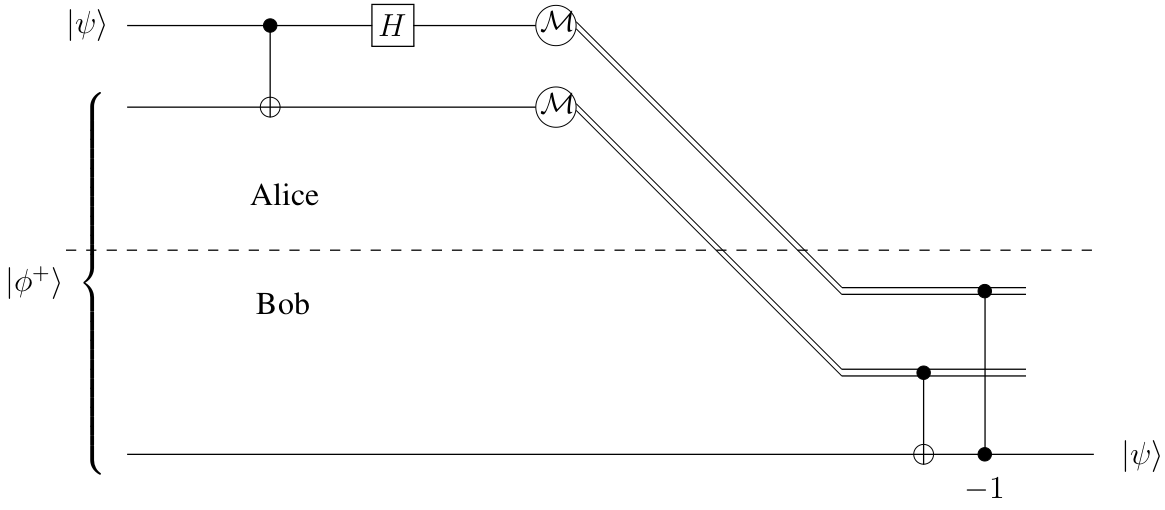
\includegraphics[width=1\textwidth]{teleportation.png}
            \caption{Quantum Teleportation Circuit}
            \label{fig:background-circuit-exampleb}
          \end{minipage}
         }
  \label{fig:background-circuit-example}
\end{figure}

\noindent\textbf{\textit{Quantum Computations and Conditionals.}} High-level quantum programming languages are usually designed to follow the \emph{QRAM model}~\cite{Knill1996}, where quantum computers are used as co-processors to classical computers. The classical computer generates descriptions of circuits to send to the quantum computer and then processes the measurement results.
Computation on a quantum value state consists of a series of \emph{quantum operations}, each of which acts on a subset of qubits in the value state. In the standard presentation, quantum computations are expressed as \emph{circuits}, as shown in \Cref{fig:background-circuit-examplea}, which constructs a circuit that prepares the Greenberger-Horne-Zeilinger (GHZ) value state \cite{Greenberger1989}, which is an $n$-qubit entangled value state of the form: $\ket{\text{GHZ}^n} = \frac{1}{\sqrt{2}}(\ket{0}^{\otimes n}+\ket{1}^{\otimes n})$.
In these circuits, each horizontal wire represents a qubit and boxes on these wires indicate quantum operations, or \emph{gates}. The circuit in \Cref{fig:background-circuit-examplea} uses $n$ qubits and applies $n$ gates: a \emph{Hadamard} (\coqe{H}) gate and $n-1$ \emph{controlled-not} (\coqe{CNOT}) gates.

% Analogous to the position and momentum representations in Schrodinger's picture of quantum mechanics, there are also two commonly used special bases in the finitely dimensional Hilbert space studied in quantum information. The computational basis refers to classical bit strings written as the tensor product of $\{\ket{0}, \ket{1}\}$, while the dual basis, or the Fourier basis, is obtained by applying \emph{quantum Fourier transformation} (QFT) on the computational basis. The computational space refers to the space spanned by the computational basis, and similarly to the dual space, although the computational and dual spaces are isomorphic to each other.  As shown by~\citet{qft-adder}, arithmetic on the computational basis can sometimes be more efficiently carried in the dual basis, which leads to the use of quantum operations in optimizing circuits with classical functionalities. 

Applying a gate to a state \emph{evolves} the state. The semantics of doing so is expressed by multiplying the state vector by the gate's corresponding matrix representation; single-qubit gates are 2-by-2 matrices, and two-qubit gates are 4-by-4 matrices. A gate's matrix must be \emph{unitary}, ensuring that it preserves the unitarity invariant of quantum states' amplitudes. An entire circuit can be expressed as a matrix by composing its constituent gates.

\noindent\textbf{\textit{Measurement.}} A \emph{measurement} operation extracts classical information from a quantum state, typically when a computation completes. Measurement collapses the state to a basis states with a probability related to the state's amplitudes. For example, measuring $\frac{1}{\sqrt{2}}(\ket{0} + \ket{1})$ in the computational basis will collapse the state to $\ket{0}$ with probability $\frac{1}{2}$ and likewise for $\ket{1}$, returning classical value 0 or 1, respectively. In all the programs discussed in this paper, we leave the final measurement operation implicit.

\noindent\textbf{\textit{Quantum Network based on Teleportation.}}
Almost all quantum network protocols are originated from the quantum teleportation algorithm \cite{PhysRevLett.70.1895}.
The circuit diagram in \Cref{fig:background-circuit-exampleb} describes a quantum teleportation circuit for communicating one qubit message between Alice and Bob. The other cases are a simple replication of the diagram.
In this algorithm, Alice sends a qubit message $\varphi$ to Bob via an entangled group $\phi^{+}$ consisting of two qubits.
Before sending the $\varphi$ qubit, Alice and Bob holds one qubit in the entangled qubit group $\phi^{+}$.
In the beginning, Alice entangles $\varphi$ with her holding $\phi^{+}$ qubit by using a CNOT gate following by a Hadamard gate.
Thus, after the two gate application, $\varphi$ joins the entangled group $\phi^{+}$.
Alice then measures her two holding qubits. This event produces two bits resulting from the measurement.
The measurement also has another conseuqnece since the three qubits are entangled;
that is, the remaining quantum information of the Alice's two qubits is pushed to store in Bob's remaining qubit.
Once Alice sends the two bits to Bob, he is able to reconstruct $\varphi$ through a proper treatment of his own qubit,
shown on the left of \Cref{fig:background-circuit-exampleb}.
In this paper, we will try to model the quantum teleportation concept
by abstracting away the details of the gates and measurement devices,
which represent a low-level circuit implementation of the quantum teleportation algorithm.


% Writing a quantum algorithm now, with SQIR (but likewise with Quipper, Pyquil, Circ, etc.). Example: Shor’s
% Write quantum parts (QPE) 
% Classical parts via library functions in meta-language (Modular multiplier)
% Refer to particular quipper functions, e.g., for adding, subtraction, etc.
% https://www.mathstat.dal.ca/~selinger/quipper/doc/Quipper-Libraries-QFTAdd.html qft_add_in_place :: QDInt -> QDInt -> Circ (QDInt, QDInt), Add one QDInt onto a second, in place; i.e. (x,y) ↦ (x,x+y). Arguments are assumed to be of equal size. This implementation follows the implementation in Thomas G. Draper's paper "Addition on a Quantum Computer" which doesn't require the use of any ancilla qubits through a clever use of the quantum Fourier transform.
% Mention Q# too
% https://github.com/microsoft/QuantumLibraries/tree/main/Numerics/src
% Maybe Scaffold:
% Write oracles via “RKQC intrinsic” functions (see sec 4.1 of https://iopscience.iop.org/article/10.1088/2058-9565/ab8c2c/pdf). The intrinsics they talk about here are super simple (swap two registers or add two registers together)
% Quipper: Write in Haskell, build_circuit, is better
% Problems to solve: Efficient compilation, verification of that compilation
% Verification: Prior work with ReverC, but only classical gates


\section{The Quantum Abstract Machine:  Syntax and Semantics} \label{sec:qam}

\begin{figure}[t]
{\small
  \[\begin{array}{llcl} 
      \texttt{Variable} & x,y \\
      \texttt{Probability} & p &\in &\Rs\\
      \texttt{Message} & m &\in& \mathbb{M}\\
    \texttt{Channel} & c &\in& \Ls\\
    \texttt{Time Stamp} & t &\in& \mathbb{T}\\
    \texttt{Label} & \alpha &::=& c.m \mid p.c.m \mid (p.c.m)^t \mid \emptyset\\
      \texttt{Configuration} & C & \\
      \texttt{Rule} & \rules & ::= & C \xrightarrow{\alpha} C \\
    \end{array}
  \]
}
\caption{Quantum Abstract Machine Syntax Table}
  \label{fig:q-pi-syntax}
\end{figure}

This section describes QAM's syntax and semantics, whose design is the abstraction of different quantum network protocols based on the observations given in \Cref{sec:introduction}.

We define QAM system to represent the transitions for any quantum network protocols, which allows programmers to define initial configurations, representing the initial programs and process environment, as well as user-definable transition rules, guiding how configurations are transitioned. A QAM system is a structure $(\Ms,\Ls,\Ts,\overline{\rules})$,
where $\Ms$ is a set of messages;
$\Ls$ is a set of channels;
$\Ts$ is a set of time stamps that forms a linear order ($<$) with $0$ being the minimum;
and $\overline{\rules}$ is a finite set of rules for guiding how configurations are transitioned. 
Any rule has the form $C_1 \xrightarrow{\alpha} C_2$, referring to that we transition configuration $C_1$ to $C_2$ via a label $\alpha$, being either emptily internal ($\emptyset$), a pair $c.m$, a triple $p.c.m$, or a quadruple $(p.c.m)^t$, where $c$ is the channel for communication, $m$ is a possibly quantum message, $p$ is the success rate of the message delivery, and $t$ is the initial time stamp of the message.

The execution in QAM is with respect to a QAM system $(\Ms,\Ls,\Ts,\overline{\rules})$ and an initial configuration $C$ that defines the input program and initial process environment.
If we collect the free metavariables ($\cn{FV}(-)$) appearing in a configuration and rule, 
the initial configuration $C$ is a \textit{ground term} without any metavariables ($\cn{FV}(C)=\emptyset$);
while $\cn{FV}(\alpha) \cup \cn{FV}(C_2)\subseteq \cn{FV}(C_1)$ for every rule $C_1 \xrightarrow{\alpha} C_2$, which is the well-formedness assumption for a QAM system.
We can define the transitions in a QAM system as follows:

\begin{definition}\label{def:labeledsystem}\rm[One QAM Transition Step]
Given a QAM system $\Cs=(\Ms,\Ls,\Ts,\overline{\rules})$ and a ground term initial configuration $C$, a transition step defining for a rule $C_1 \xrightarrow{\alpha} C_2 \in \overline{\rules}$ on $C$ is given as:
\begin{itemize}
\item We find a substitution $\sigma$ mapping every metavariable in $C_1$ to a term, such that $\sigma(C_1)=C$, where we substitute metavariables $x$ in $C_1$ with the mapped terms as $\sigma(x)$.
\item The result label and configuration by applying the rule is $\sigma(\alpha)$ and $\sigma(C_2)$.
\end{itemize}
\end{definition}

\Cref{def:labeledsystem} provides an abstraction of transitions in QAM, where the details configurations and rules are parameterized as some abstract objects. Below, we provide step by step instantiation of configurations and rules to capture different quantum network protocol behaviors. 

\ignore{
      \texttt{Singleton Action} & A & ::= & \qsend{p}{c}{m}^{t?} \mid \qrev{c}{x} \\
      \texttt{Process} & P,Q & ::= & 0 \mid A.P \mid \parl{P}{Q} \mid \comp{P} \\
      \texttt{Relations} & R & \in & \Ls \times \Ls \times \Rs \\
      \texttt{Predicate Action} & \alpha & ::= & \qsend{p}{c}{m}^t \mid (c,c,\qsend{p}{c}{m}^t) \\
      \texttt{Objects} & \Os \\
      \texttt{Custom Cell} & \varphi,\psi & ::= & \pcell{P}{n}{c} \mid \qcell{\Os}{c}\\
      \texttt{Configuration} & C & ::= & \varphi^* \qcell{R}{\cn{rel}} \qcell{t}{\cn{gt}}
                             \qcell{\alpha}{\cn{comm}} \pcell{\cn{bool}}{t}{\cn{pred}} \psi^* \\
}

\subsection{Intra-Destination Process Communication} \label{sec:qamsyntax}

\begin{figure}[t]
{\small
$\textcolor{blue}{\text{Syntax:}}\\$
  \[\begin{array}{llcl} 
    \texttt{Singleton Action} & A & ::= & \qsend{p}{c}{m}^{t?} \mid \qrev{c}{x}\\
      \texttt{Process} & P,Q & ::= & 0 \mid A.P \mid \parl{P}{Q} \mid \parp{P}{Q}\mid \comp{P} \\
      \textcolor{red}{\texttt{Configuration First Instant}} & \textcolor{red}{C} & \textcolor{red}{::=} & \textcolor{red}{\overline{P}} \\
    \end{array}
  \]

$\textcolor{blue}{\text{Semantics:}}\\$
  \begin{mathpar}
\mprset{flushleft}

   \inferrule[Heating]{}
       {\parl{P}{Q} \longrightarrow \pard{P}{Q}}

   \inferrule[Cooling]{}
       {\pard{P}{Q} \longrightarrow \parl{P}{Q}}

   \inferrule[ID]{}
       {\pard{0}{P} \longrightarrow P}

  \inferrule[CL]{}
      {\parp{P}{Q} \longrightarrow P}

  \inferrule[CR]{}
      {\parp{P}{Q} \longrightarrow Q}

  \inferrule[PC]{}
      { \pard{\qsend{p}{c}{m}^t.Q}{ \qrev{c}{x}.P}
           \xrightarrow{(p.c.m)^t} \pard{Q}{P[m/x]}}

   \inferrule[MT]{}
       {\comp{P} \longrightarrow \pard{P}{\comp{P}}}
      
   \inferrule[NT]{}
       {\comp{P} \longrightarrow 0}
  \end{mathpar}
}
\caption{Single-party process communication syntax and semantics. The $?$ mark in $\qsend{p}{c}{m}^{t?}$ means that the time stamp $t$ can be omitted.}
  \label{fig:q-pi-semantics1}
\end{figure}

We first investigate the quantum communication between parties in a single location.
Essentially, quantum teleportation can be split into two parts: 1) using quantum swap mechanism to build the channel for communicating Alice and Bob; and 2) Bob reproduces the quantum message by a piece of the message and two classical bits.
Here, we model (1) along with the modeling for quantum routing because they are essentially the same, while we model the intra-destination level communication mainly focuses on Bob's receipt of the quantum message, which can be modeled based on the CHEM mechanism in \Cref{fig:q-pi-semantics1}.

The syntax of the intra-destination level communication is enlightened by $\Pi$-calculus, as we instantiate QAM configurations as a multiset of processes $\overline{P}$, referring to the red part in \Cref{fig:q-pi-semantics1}.
Each single process action is either a message sending $\qsend{p}{c}{m}^{t}$, meaning that a message $m$ is sent through the channel $c$ with the success probability rate $p$ initialized at the time stamp $t$, or a message receipt $\qrev{c}{x}$, referring to that a message is received through the channel $c$ and represented as variable $x$ in the following computation.
The time stamp $t$ in a message sending operation can be omitted as $\qsend{p}{c}{m}$, meaning that an initial time stamp will be generated when the message is sent out from its starting place.

A process can be an empty process $0$, a process ($A.P$) executing a singleton action with continuation, a parallel process ($\parl{P}{Q}$) of two parties $P$ and $Q$, a choice operation($\parp{P}{Q}$), and a replication process $\comp{P}$ referring to that $P$ can repeatedly happen zero or multiple times. As an instance, process $Q$ in $\parl{\qact{\qsend{0.5}{\cn{Ann}}{m}^0}{P}}{\qact{\qrev{\cn{Ann}}{x}}{Q}}$ represents that \cn{Ann} receives a message $m$, initializing at time $0$, from the process $P$ in a $50\%$ change; after $m$'s receipt, the message is represented as variable $x$ in the continuation of process $Q$.

The intra-destination level semantics in \Cref{fig:q-pi-semantics1} is inherited from CHEM.
Through the \rulelab{Heating} rule, a parallel process $\parl{P}{Q}$ is dissolved to a multiset ($\pard{P}{Q}$) containing two elements $P$ and $Q$, ready for semantic evaluation; while the \rulelab{Cooling} rule merges two elements in a multiset ($\pard{P}{Q}$) as a parallel process. Rules \rulelab{Heating}, \rulelab{Cooling}, and \rulelab{ID} captures the implicit associativity, commutativity, and identity equational properties for QAM processes, so that any two processes in the process multiset might communicate, without syntactic barriers. For example, in a multiset, rule \rulelab{PC} defines the behavior of a sender process, on the left, communicating an action $\qsend{p}{c}{m}^t.Q$ with a receiver process $\qrev{c}{x}.P$, on the right, and resulting in the two multiset elements $\pard{Q}{P[m/x]}$, indicating that process $P$ consumes the message $m$ as variable $x$ in the following continuation. The above three rules allow us not to care about the positions of the sender and receiver in the multiset.

Rules \rulelab{CL} and \rulelab{CR} define conditional choice operations. For example, if we have:
$\parl{\qact{\qsend{0.5}{\cn{Ann}}{m}^0}{P}}{\parp{\qact{\qrev{\cn{Ann}}{x}}{Q}}{\qact{\qrev{\cn{Ann}}{x}}{Q'}}}$, 
we can nondeterministically choose the receiver process as $Q$ or $Q'$:
$\parl{\qact{\qsend{0.5}{\cn{Ann}}{m}^0}{P}}{\qact{\qrev{\cn{Ann}}{x}}{Q}}$
or
$\parl{\qact{\qsend{0.5}{\cn{Ann}}{m}^0}{P}}{\qact{\qrev{\cn{Ann}}{x}}{Q'}}$.
Rules \rulelab{MT} and \rulelab{NT} define the nondeterministic behavior of a replication operation $\comp{P}$,
i.e., to replicate zero or more processes $P$. In defining quantum network protocols, 
such operations represent the concept of repeatedly sending a same message to ensure success rate for message delivery.
We will explain the utility shortly in \Cref{sec:add-prop}.

\subsection{QAM Semantics For Inter-Destination Communication} \label{sec:qamsyntax}

As an example of the QAM syntax, the above configuration defines the initial program state for sending a message $c.m$ from $\cn{Cat}$ to $\cn{Dan}$ via the router $r_1$, as part of the communication in \Cref{fig:q-pi-example}. Initially, the relation cell stores the connectivity between \cn{Cat}, \cn{Dan}, and $r_1$, with the success rates. 
The global time is initialized as $0$ in the \cn{gt} cell, and the predicate cell has a fixed value $\texttt{false}$.
The message ($\qsend{1}{c}{m}$) sent from \cn{Cat} has an initial probability value $1$.
Node $r_0$ acts as a intermediate router, so it only contains the unit process $0$, and \cn{Dan} is waiting on receiving a message ($\qrev{c}{x}.0$). 

\begin{figure}[t]
{\small
  \begin{mathpar}
\mprset{flushleft}
   \inferrule[GC]{}
       {\Cellb{\qsend{p}{c}{m}^t}{i}{c_1}\Cella{P}{j}{c_2} \qcell{\{(c_1,c_2,p')\}\cup R}{\cn{rel}}\qcell{t'}{\cn{gt}}
        \qcell{\emptyset}{\cn{comm}}\pcell{b}{\_}{\cn{pred}}
       \\\\\qquad\qquad \longrightarrow \Cellb{}{i-}{c_1}\Cella{\qsend{p*p'}{c}{m}^{t}\texttt{|}P}{j-}{c_2}
              \qcell{\{(c_1,c_2,p')\}\cup R}{\cn{rel}}\qcell{t'}{\cn{gt}}
               \qcell{(c_1,c_2,\qsend{p}{c}{m}^t)}{\cn{comm}}\pcell{b}{t'}{\cn{pred}}}

\ignore{
   \inferrule[GenQubit]{}
       {\Cella{P}{n,t'}{a}\qcell{t}{\cn{gt}}\longrightarrow \Cella{P}{n+,t}{a}\qcell{t}{\cn{gt}}}\;\;\texttt{when}\;t \texttt{|} \beta\wedge t' < t
}

   \inferrule[CT]{}
       {\Cellb{\qsend{p}{c}{m}}{i}{c_1}\qcell{t}{\cn{gt}} \longrightarrow \Cellb{\qsend{p}{c}{m}^t}{i}{c_1}\qcell{t}{\cn{gt}}}

   \inferrule[MT]{}
       {\comp{P} \longrightarrow \parl{P}{\comp{P}}}
      
   \inferrule[NT]{}
       {\comp{P} \longrightarrow 0}

  \inferrule[PC]{}
      { \Cellb{\qsend{p}{c}{m}^t\texttt{|} \qrev{c}{x}.P}{n}{c}\qcell{t'}{\cn{gt}}\qcell{\emptyset}{\cn{comm}}\pcell{b}{\_}{\cn{pred}}
           \longrightarrow
         \Cellb{P[m/x]}{n}{c}\qcell{t'}{\cn{gt}}\qcell{\qsend{p}{c}{m}^t}{\cn{comm}}\pcell{b}{t'}{\cn{pred}}}
                  
  \inferrule[Com]{}
      { \qcell{t'}{\cn{gt}}\qcell{\qsend{p}{c}{m}^t}{\cn{comm}}\pcell{\cn{true}}{t'}{\cn{pred}}
           \xrightarrow{p.c.m}  
         \qcell{t'+}{\cn{gt}}\qcell{\emptyset}{\cn{comm}}\pcell{\cn{false}}{t'}{\cn{pred}} } 

  \inferrule[FC]{}
      { \qcell{t}{\cn{gt}}\qcell{(c_1,c_2,A)}{\cn{comm}}\pcell{\cn{true}}{t}{\cn{pred}}
           \longrightarrow
         \qcell{t+}{\cn{gt}}\qcell{\emptyset}{\cn{comm}}\pcell{\cn{false}}{t}{\cn{pred}} } 

  \end{mathpar}
}
\caption{Quantum Pi Semantics. $\beta$, $\mu$, and $\nu$ are globally defined for the qubit generation period, the message threshold probability, and message sending finished threshold. $\Cella{P}{n}{a}$ refers to that the $t$ in $\Cella{P}{n,t}{a}$ is omitted in the rule.}
  \label{fig:q-pi-semantics}
\end{figure}

\ignore{
\begin{figure}[t]
{\small
{\hspace*{-2em}
\begin{tikzpicture}[align=center,node distance=1.5cm and -1cm, thick] 
\node (1) {S$\langle\{(a,r_1,0.5), (a,r_2,0.5)\}\cup$R$\rangle$}; 
\node (2) [below left= of 1] {$\Cella{0}{9}{a}$ $\Cella{\qsend{0.5}{c}{m}|0}{9}{r_1}$... $\langle\{(r_1,r_4)\}\cup$R$\rangle$}; 
\node (3) [below right= of 1] {\text{\ \ \ \ \ \ }$\Cella{0}{9}{a}$ $\Cella{\qsend{0.5}{c}{m}|0}{9}{r_2}$..., $\ccell{\{(r_2,r_3)\}\cup\text{R}}$}; 
\node (4) [below of=2] {$\Cella{0}{8}{r_1}$ $\Cella{\qsend{0.25}{c}{m}|0}{9}{r_4}$... $\langle\{(r_4,b)\}\cup$R$\rangle$};
\node (5) [below of=3] {\text{\ \ \ \ \ \ }$\Cella{0}{8}{r_2}$ $\Cella{\qsend{0.25}{c}{m}|0}{9}{r_3}$..., $\ccell{\{(r_3,r_4)\}\cup\text{R}}$};
\node (6) [below of=4] {$\Cella{0}{8}{r_4}$ $\Cella{\qsend{0.125}{c}{m}|\qrev{c}{x}.0}{9}{b}$... $\ccell{\text{R}}$};
\node (7) [below of=5] {\text{\ \ \ \ \ \ \ \ \;}$\Cella{0}{8}{r_3}$ $\Cella{\qsend{0.125}{c}{m}|0}{9}{r_4}$..., $\ccell{\{(r_4,b)\}\cup\text{R}}$};
\node (8) [below of=6] {$\Cella{0}{9}{b}$... $\ccell{\text{R}}$};
\node (9) [below of=7] {\text{\ \ \ \ \ \ \ \ }$\Cella{0}{8}{r_4}$ $\Cella{\qsend{0.0625}{c}{m}|\qrev{c}{x}.0}{9}{b}$..., $\ccell{\text{R}}$};
\node (10) [below of=9] {\text{\ \ \ \ \ \ }$\Cella{0}{n}{b}$... $\ccell{\text{R}}$};
\draw[->] (1) -- node[midway, above left] {} (2); 
\draw[->] (1) -- node[midway, above right] {} (3); 
\draw[->] (2) -- node[midway, right] {} (4); 
\draw[->] (4) -- node[midway, right] {} (6);
\draw[->] (6) -- node[midway, right] {$0.125.c.m$} (8); 
\draw[->] (3) -- node[midway, right] {} (5); 
\draw[->] (5) -- node[midway, right] {} (7); 
\draw[->] (7) -- node[midway, right] {} (9);
\draw[->] (9) -- node[midway, right] {$0.0625.c.m$}  (10); 
\end{tikzpicture} 
}
}
\caption{Quantum Machine Transitions for \Cref{fig:q-pi-example}}
  \label{fig:q-pi-example1}
\end{figure} 
}

\begin{figure}[t]
{\small
\begin{center}
\begin{tikzpicture}[node distance={1cm}, thick, main/.style = {draw, circle}] 
\node[main] (1) {\cn{Ann}}; 
\node[main] (2) [right of=1] {$r_1$};
\node[main] (3) [right of=2] {$r_4$};
\node[main] (4) [right of=3] {\cn{Bob}};
\node[main] (5) [above right=0.5cm and 1.5cm of 1] {$r_2$};
\node[main] (6) [right of=5] {$r_3$};
\node[main] (7) [below of=1] {\cn{Cat}};
\node[main] (8) [below of=3] {\cn{Dan}};
\draw[-] (1) --  (2);
\draw[-] (2) --  (3);
\draw[-] (3) --  (4);
\draw[-] (1) --  (5);
\draw[-] (5) --  (6);
\draw[-] (6) --  (3);
\draw[-] (7) --  (2);
\draw[-] (2) --  (8);
\end{tikzpicture}
\end{center}
}
\caption{Example Path Connectivity}
  \label{fig:q-pi-example}
\end{figure}

\subsection{Semantics} \label{sec:qamsemantics}

Defining protocol systems might require the extension of semantic rule set to include specific behaviors.
We provide a meta level rule declaration operation ($\decl{\rules}{\Cs}$), allowing users to declare a new rule $\rules$ used in the system $\Cs$. 

{\footnotesize
\[
\Cella{\qsend{1}{c}{m}}{10}{\cn{Cat}}\Cella{0}{10}{r_1}
\Cella{\qrev{c}{x}.0}{10}{\cn{Dan}} 
\qcell{\{(\cn{Cat},r_1,0.5), (r_1,\cn{Dan},0.5)\}}{\cn{rel}}
\qcell{\emptyset}{\cn{comm}}
\pcell{\texttt{false}}{0}{\cn{pred}}
\qcell{0}{\cn{gt}}
\]
}

To describe the behaviors of a network system, every QAM system comes with a configuration $C$
containing two different kinds of cells --- process and content cells.
A configuration might contain one or more process cells $\pcell{P}{n}{c}$, representing the execution maltreated process of a local node with name $c$, such as the $\cn{Ann}$ and $r_1$ nodes in \Cref{fig:q-pi-example},
and $n$ is the available qubit resource in the node.
A multi-threaded process $P$ is the program actions that node $c$ can perform, which has similar syntax as $\Pi$-calculus.
Each process might contain multiple threads competing for executions, which are separated by a parallel operation $\cn{|}$.
Each single thread is a sequence of singleton actions that ends at the unit process $0$,
and $\comp{P}$ is a replication process that repeatedly executes the process $P$, 
which is used for resending messages, explained in \Cref{sec:qamsemantics}.

In QAM, a parallel process of a message sending and receipt, $\parl{\qact{\qsend{p}{c}{m}^t}{P}}{\qact{\qrev{c}{x}}{Q}}$,
causes the process to transit to $\parl{P}{Q[m/x]}$, which is similar to the $\Pi$-calculus semantics.
On the other hand, a parallel of two message sending, $\parl{\qact{\qsend{p}{c}{m}^t}{P}}{\qsend{p'}{c'}{m'}^{t'}{P'}}$,
refers to that the two operations are competing to transmit the message outside of the node, possibly to other destinations.

The content cells act as control units for storing environment information for executing a QAM system.
Users are able to define their own content cell by instantiating object types $\Os$ to different user-defined types.
In QAM, we require at least four kinds of content cells: 
1) $\qcell{R}{\cn{rel}}$ is a relation cell defining the probability value to send out one message from a node to the other;
2) $\qcell{t}{\cn{gt}}$ is a global clock cell storing the global time stamp;
3) $\qcell{A}{\cn{comm}}$ is a communication cell storing the message about to communicate;
and 4) $\pcell{\cn{bool}}{t}{\cn{pred}}$ is a predicate cell 
determining if a message communication can happen ($\texttt{true}$ in the cell) or not ($\texttt{false}$ in the cell) at time $t$.

The QAM semantics is given in terms of the definition of a QAM system,
which is a structure $(\Ms,\Ls,\Ts,C,\overline{\rules})$,
where $\Ms$ is a set of messages;
$\Ls$ is a set of channels containing at least $\cn{rel}$, $\cn{comm}$, $\cn{gt}$, and $\cn{pred}$;
$\Ts$ is a set of time stamps that forms a linear order ($<$) with $0$ being the minimum;
$C$ is the configuration containing different cells that represent the nodes with processes and environment for the system, at least containing cell $\cn{rel}$, $\cn{comm}$, $\cn{gt}$, and $\cn{pred}$, mentioned in \Cref{sec:qamsyntax};
and $\overline{\rules}$ is a set of rule for guiding how the configuration is transited, at least contain rules \rulelab{CT},\rulelab{GC}, \rulelab{MT}, \rulelab{NT}, \rulelab{PC}, and \rulelab{Com} in \Cref{fig:q-pi-semantics}. 

QAM is flexible enough to define most quantum network/security protocols 
through the ability to extend rules by the rule declaration operation in \Cref{fig:q-pi-syntax}.
Every rule set must contain the six rules listed in \Cref{fig:q-pi-semantics},
because they represent the universally sound facts about multiparty quantum communication. 
We first discuss these six rules through the example configuration at the end of \Cref{sec:qamsyntax}. 
For showing the consecutive transitions of a system, there must be additional rules for
granting every step of transition by turning the \cn{pred} cell's content to be \cn{true}.
Here, we first assume our example system includes the simplest granting rule by assigning \cn{true} to the \cn{pred} cell if the global time stamps in the \cn{gt} and \cn{pred} cells matched, as:

{\small
  \begin{mathpar}
   \inferrule[Grant]{}
       {\qcell{t}{\cn{gt}}\pcell{\cn{false}}{t}{\cn{pred}} \longrightarrow \qcell{t}{\cn{gt}}\pcell{\cn{true}}{t}{\cn{pred}}}
\end{mathpar}
}

In QAM, there are mainly two groups of rules, finishing the tasks of transmitting a message from a starting node to its destination via many middle routers and delivering the message in the destination.
Each group can be divided into a consecutive three kinds of rule applications: 1) we finish the major functionality of the task and move necessary information to the \cn{comm} and \cn{pred} cells for granting; 2) one or more granting rules are applied on the system to check if the task is finished correctly; and 3) we clean up the task information from the \cn{comm} and \cn{pred} cells and update the global clock to finalize the task execution.

In transmitting a message from a starting node to its destination,
we have the rule applications \rulelab{GC} and \rulelab{FC} for step (1) and (3) above, with some possible granting rules, such as rule \rulelab{Grant} above.
Rule \rulelab{GC} defines the message transmission behavior that might be an intermediate router node, with the consumption of a qubit in each of the parties and a slot time change happening in the global clock.
The $...$ operation in cell $a$ refers to that there might 
be other paralleled processes associated in the process cell, but we disregard them.
In rule \rulelab{GC}, it also moves the necessary information, such as the sender and receiver channel names as well as the message, in the \cn{comm} cell with the update of the time stamp $t'$ in the \cn{pred} cell to be the current global time,
indicating that at the current point, the system conveys a message from a node to another.
After an intermediate granting step, rule \rulelab{FC} is applied on a configuration to empty the \cn{comm} cell, initialize the \cn{pred} cell by putting an \cn{false} value, and increment the global clock.
Additionally, rule \rulelab{CT} generates a time stamp for a message that is about to send out.

{\footnotesize
\[
\begin{array}{ll}
\longrightarrow\;\;
\Cella{\qsend{1}{c}{m}^0}{10}{\cn{Cat}}\Cella{0}{10}{r_1}
\Cella{\qrev{c}{x}.0}{10}{\cn{Dan}} 
\qcell{\{(\cn{Cat},r_1,0.5), (r_1,\cn{Dan},0.5)\}}{\cn{rel}}
\qcell{\emptyset}{\cn{comm}}
\pcell{\texttt{false}}{0}{\cn{pred}}
\qcell{0}{\cn{gt}}
&
(\rulelab{CT})
\\[0.2em]
\longrightarrow\;\;
\Cella{0}{9}{\cn{Cat}}\Cella{A}{9}{r_1}
\Cella{\qrev{c}{x}.0}{10}{\cn{Dan}} 
\qcell{R}{\cn{rel}}
\qcell{(\cn{Cat},r_1,A)}{\cn{comm}}
\pcell{\texttt{false}}{0}{\cn{pred}}
\qcell{0}{\cn{gt}}
&
(\rulelab{GC})
\\[0.2em]
\longrightarrow\;\;
\Cella{0}{9}{\cn{Cat}}\Cella{A}{9}{r_1}
\Cella{\qrev{c}{x}.0}{10}{\cn{Dan}} 
\qcell{R}{\cn{rel}}
\qcell{(\cn{Cat},r_1,A)}{\cn{comm}}
\pcell{\texttt{true}}{0}{\cn{pred}}
\qcell{0}{\cn{gt}}
&
(\rulelab{Grant})
\\[0.2em]
\longrightarrow\;\;
\Cella{0}{9}{\cn{Cat}}\Cella{A}{9}{r_1}
\Cella{\qrev{c}{x}.0}{10}{\cn{Dan}} 
\qcell{R}{\cn{rel}}
\qcell{\emptyset}{\cn{comm}}
\pcell{\texttt{false}}{0}{\cn{pred}}
\qcell{1}{\cn{gt}}
&
(\rulelab{FC})
\\[0.2em]
\longrightarrow\;\;
\Cella{0}{9}{\cn{Cat}}\Cella{0}{8}{r_1}
\Cella{\parl{A'}{\qrev{c}{x}.0}}{9}{\cn{Dan}} 
\qcell{R}{\cn{rel}}
\qcell{(r_1,\cn{Dan},A')}{\cn{comm}}
\pcell{\texttt{false}}{1}{\cn{pred}}
\qcell{1}{\cn{gt}}
&
(\rulelab{GC})
\end{array}
\]
}
{\footnotesize
\begin{center}
$R\triangleq\{(\cn{Cat},r_1,0.5), (r_1,\cn{Dan},0.5)\}
\qquad
A\triangleq\qsend{0.5}{c}{m}^0
\qquad
A'\triangleq\qsend{0.25}{c}{m}^0$
\end{center}
}

The above transitions evolves the configuration in \Cref{sec:qamsyntax}. We first apply rule \rulelab{CT} to attach the current time $0$ to the message to send as $\qsend{1}{c}{m}^0$; then, apply rule \rulelab{GC}. The message $\qsend{1}{c}{m}^0$ in cell \cn{Cat} is transmitted to the $r_1$ cell with the new probability $0.5$, meaning that only $50\%$ change this communication is guaranteed.
This can happen because there is a defined relation tuple $(\cn{Cat},r_1,0.5)$ in the relation cell $\cn{rel}$. During the process, the qubit resources in $\cn{Cat}$ and $r_1$ both reduce one, and the global clock is updated. 
It is worth noting that 
we associate the parallel process $\cn{|}$ with identity, associativity, and commutativity equational rules, 
such that $\parl{P}{0}=P$, $\parl{(\parl{P}{Q})}{Q'}=\parl{P}{(\parl{Q}{Q'})}$, and $\parl{P}{Q}=\parl{Q}{P}$.
In the above case, $\qsend{0.5}{c}{m}^0$ can be viewed as $\parl{\qsend{0.5}{c}{m}^0}{0}$.
We then apply rule \rulelab{Grant} to put a \cn{true} value in the \cn{pred} cell and the \rulelab{FC} rule application cleans up the cells, so the transition of the message from node $r_1$ to \cn{Dan} can happen through the last \rulelab{GC} rule application.

{\footnotesize
\[
\begin{array}{lll}
&\Cella{0}{9}{\cn{Cat}}\Cella{0}{8}{r_1}
\Cella{\parl{A'}{\qrev{c}{x}.0}}{9}{\cn{Dan}} 
\qcell{R}{\cn{rel}}
\qcell{\emptyset}{\cn{comm}}
\pcell{\texttt{false}}{1}{\cn{pred}}
\qcell{2}{\cn{gt}}
\\[0.2em]
\longrightarrow
&
\Cella{0}{9}{\cn{Cat}}\Cella{0}{8}{r_1}
\Cella{0}{9}{\cn{Dan}} 
\qcell{R}{\cn{rel}}
\qcell{A'}{\cn{comm}}
\pcell{\texttt{false}}{2}{\cn{pred}}
\qcell{2}{\cn{gt}}
&
(\rulelab{PC})
\\[0.2em]
\longrightarrow
&
\Cella{0}{9}{\cn{Cat}}\Cella{0}{8}{r_1}
\Cella{0}{9}{\cn{Dan}} 
\qcell{R}{\cn{rel}}
\qcell{A'}{\cn{comm}}
\pcell{\texttt{true}}{2}{\cn{pred}}
\qcell{2}{\cn{gt}}
&
(\rulelab{Grant})
\\[0.2em]
\xrightarrow{0.25.c,m}
&
\Cella{0}{9}{\cn{Cat}}\Cella{0}{8}{r_1}
\Cella{0}{9}{\cn{Dan}} 
\qcell{R}{\cn{rel}}
\qcell{\emptyset}{\cn{comm}}
\pcell{\texttt{false}}{2}{\cn{pred}}
\qcell{3}{\cn{gt}}
&
(\rulelab{Com})
\end{array}
\]
}
{\footnotesize
\begin{center}
$R\triangleq\{(\cn{Cat},r_1,0.5), (r_1,\cn{Dan},0.5)\}
\qquad
A'\triangleq\qsend{0.25}{c}{m}^0$
\end{center}
}

For delivering a message in the destination,
rules \rulelab{PC} and \rulelab{Com} define the steps except the intermediate granting step.
Rule \rulelab{PC} is applicable if the sending operation is already in its destination cell, and being paralleled with a same-channel message receipt process $\qrev{c}{x}.P$. After applying the rule, the message is processed as $P[m/x]$, and we also move the message $\qsend{p}{c}{m}^t$ to the communication cell $\cn{comm}$ with the current time stamp $t'$, so further user-defined rules can be applied on the message.
The above example first provides an \rulelab{PC} rule application showing the exactly procedure above, i.e, the message is moved to the \cn{comm} cell with the current global time $2$.
After the granting step,
a \rulelab{Com} rule application processes the delivered message $\qsend{p}{c}{m}^t$ by removing it from the $\cn{comm}$ cell if the predicate cell $\cn{pred}$ is $\texttt{true}$. The processing refers to making the message a transition label $p.c.m$ appearing in the transition,
so the message delivery is publicized. Other than applying rule \rulelab{Com}, all other rule applications are considered to be internal communications. 
In the above example, the last \rulelab{Com} rule application removes the message from the cell with a publicized transition label $0.25.c,m$. 

Rules \rulelab{MT} and \rulelab{NT} define the behaviors of the replication $\comp{P}$.
The former suggests that a process can be replicated as many as we want, while the latter one refers to that a replication process can non-deterministically terminates.
In quantum communication, message deliveries are always associated with a success rate,
which indicates that users might be interested in repeatedly sending a message until some success rate assurance is guaranteed.
We will see an example success rate guarantee mechanism by using the replication operations with additional user-defined rules in \Cref{sec:add-prop}.

\noindent\textbf{Extension of Rules.}
The rule set $\overline{\rules}$ is extendable by user-defined rules, 
such that if a user declares the statement $\decl{\rules_1}{...\; \decl{\rules_n}{C_0}}$
in the QAM system $(\Ms,\Ls,\Ts,C,\overline{\rules})$, $C=C_0$ and $\overline{\rules}=\{\rules_1,...\rules_n,\rulelab{CT},\rulelab{GC},\rulelab{MT},\rulelab{NT}, \rulelab{PC},\rulelab{Com}\}$.

Permitting user-defined rules allows the definitions of different protocol guarantees in QAM,
which are useful in evaluating different performance merits of different protocols,
while rules in \Cref{fig:q-pi-semantics} establish the semantic basis of quantum network communication.
As the \rulelab{Grant} rule example above, the guarantees are established by evaluating different predicates in the \cn{pred} cell,
which we name granting steps in handling the tasks of conveying and delivering messages.
Here, we discuss how to guarantee the on-time message delivery in the QPass/QCast protocols \cite{10.1145/3387514.3405853},
which is a property that people tried to guarantee in these these protocols, but was not established formally \cite{10.1145/3387514.3405853}.

A key observation in quantum network is that qubit messages have short liftime,
so the above quantum protocols developed complicated algorithms to guarantee the high delivery rates for quantum messages.
If a message is not delivered in time, its quantum state is decohered and its information loses.

{\footnotesize
\[
\begin{array}{l}
\decl{\pcell{\qsend{p}{c}{m}^t}{t'}{\cn{comm}}\qcell{b}{\cn{pred}}\qcell{f}{\cn{tp}} 
     \longrightarrow \pcell{\qsend{p}{c}{m}^t}{t'}{\cn{comm}}\qcell{f(t,t')}{\cn{pred}}\qcell{f}{\cn{tp}}}{}
\\[0.2em]
\qquad
\Cella{\qsend{1}{c}{m}^0}{10}{\cn{Cat}}\Cella{0}{10}{r_1}
\Cella{\qrev{c}{x}.0}{10}{\cn{Dan}} 
\qcell{R}{\cn{rel}}
\pcell{\emptyset}{0}{\cn{comm}}
\qcell{\texttt{false}}{\cn{pred}}
\qcell{0}{\cn{gt}}
\qcell{\lambda\;(t,t')\,.\,t'-t<5}{\cn{tp}}
\end{array}
\]
}
{\footnotesize
\begin{center}
$R\triangleq\{(\cn{Cat},r_1,0.5), (r_1,\cn{Dan},0.5)\}$
\end{center}
}

To guarantee the property, we add a new cell $\cn{tp}$ and declare a new rule above (let's call it rule \rulelab{TP}).
Every time when an action is in the \cn{comm} cell, which we know rule \rulelab{PC} is applied prior to the state, we apply the function $f$ in the new content cell \cn{tp} to the two time stamps $t$ and $t'$, and check if the message starting time $t$ and its delivery time $t'$ is within a threshold.
In the configuration setting, function $f$ is defined as a lambda abstraction $\lambda\;(t,t')\,.\,t'-t<5$ and it takes two time stamps and checks if $t'-t$ is less than the threshold number $5$. In addition, we can rewrite the \rulelab{Grant} rule below to only grant transitions for conveying messages; in such case, the \cn{comm} cell contains a tuple $(c_1,c_2,A)$.  

{\small
  \begin{mathpar}
   \inferrule[Grant]{}
       {\qcell{t}{\cn{gt}}\qcell{(c_1,c_2,A)}{\cn{comm}}\pcell{\cn{false}}{t}{\cn{pred}} \longrightarrow \qcell{t}{\cn{gt}}\qcell{(c_1,c_2,A)}{\cn{comm}}\pcell{\cn{true}}{t}{\cn{pred}}}
\end{mathpar}
}

After we declare rule \rulelab{TP} and the new configuration, we essentially create a new QAM system $(\Ms,\Ls,\Ts,C',\overline{\rules'})$,
where $C'$ is the new declared configuration and the rule set $\overline{\rules'}$ contains the six rules in \Cref{fig:q-pi-semantics}, rule \rulelab{Grant} above, as well as rule \rulelab{TP}.
In the execution example above, after applying rule \rulelab{PC}, the \cn{comm} cell becomes $\pcell{\qsend{0.25}{c}{m}^0}{2}{\cn{comm}}$ with the starting time stamp $0$ and the delivery time stamp $2$.
By applying rule \rulelab{TP}, the expression $2-0 < 5$ results in \texttt{true}, which grants the message transition for the following \rulelab{Com} rule application. 
However, if we set the threshold to be $2$, such as having the function definition $\lambda\;(t,t')\,.\,t'-t<2$ in the \cn{tp} cell of the above configuration, the expression $2-0 < 2$ results in \texttt{false}, which means that the following \rulelab{Com} rule is not applicable.
The system might be stuck because there is no rule to empty the \cn{comm} cell, which can be classified as a failure due to the violation of the delivery time guarantee. 












\section{Behavioral Refinement and Equivalence} \label{sec:refinement}

Here, we define QAM trace refinement relations, where two QAM systems are equivalent if the same sequences of actions can be performed
from their respective initial states.
Essentially, a QAM system $(\Ms,\Ls,\Ts,C,\overline{\rules})$
can be viewed as a tuple of four fixed sets $\Cs=(\Ms,\Ls,\Ts,\overline{\rules})$
and a configuration $C$ representing the initial program state.
Each rule in $\overline{\rules}$ is a label transition relation $C_1 \xrightarrow{\alpha} C_2$,
where $C_1$ and $C_2$ are configurations representing the states
before and after the rule application, and $\alpha$ is either empty or $p.c.m$.
If we collect the free metavariables ($\cn{FV}(-)$) appearing in a configuration and rule, 
the initial configuration $C$ is a \textit{ground term} without any metavariables ($\cn{FV}(C)=\emptyset$);
while $\cn{FV}(\alpha) \cup \cn{FV}(C_2)\subseteq \cn{FV}(C_1)$ for every rule, which is the well-formedness assumption for a QAM system.
We can define the transitions in a QAM system as follows:



Based on the transition step definition, we define QAM traces as an inductive set below. Given a QAM system tuple $\Cs=(\Ms,\Ls,\Ts,\overline{\rules})$, a ground term configuration $C$ is \textit{stuck}, if and only if no rules in $\overline{\rules}$ can be applied on $C$ for a transition step. We also refer to $C \longrightarrow^* C'$ as configuration $C$ transitioning to $C'$, based on the rules in $\Cs$, via several internal steps (steps having no labels).

\begin{definition}\label{def:traces}\rm[QAM Traces]
Given a QAM system tuple $\Cs=(\Ms,\Ls,\Ts,\overline{\rules})$, traces of a configuration $C$ on the tuple is defined as an inductive set $\Tts(\Cs,C)$ of label sequences as:

\begin{itemize}
\item If $C \longrightarrow^* C'$ and $C'$ is stuck, $\Tts(\Cs,C)=\emptyset$.
\item If $C \longrightarrow^* C' \xrightarrow{p.c.m} C''$ and $C'$ is stuck, $\Tts(\Cs,C)=(c.m)::\Tts(\Cs,C'')$, i.e., $(c.m)::\Tts(\Cs,C'')$ is a new set that for all sequence $\xi \in \Tts(\Cs,C'')$, $(c.m)::\xi \in (c.m)::\Tts(\Cs,C'')$ and $::$ is a sequence concatenation operation.
\end{itemize}
\end{definition}

With the trace definition above, we can then define a trace refinement relation between two different QAM systems with tuples $\Cs=(\Ms,\Ls,\Ts,\overline{\rules})$ and $\Cs=(\Ms',\Ls',\Ts',\overline{\rules'})$, as well as initial configurations $C$ and $C'$.

\begin{definition}\label{def:traceeq}\rm[QAM Trace Refinement]
Given two QAM system tuples $\Cs=(\Ms,\Ls,\Ts,\overline{\rules})$ and $\Cs=(\Ms',\Ls',\Ts',\overline{\rules'})$, and initial configurations $C$ and $C'$,  we say that $(\Cs,C)$ trace refines $(\Cs',C')$, written as $(\Cs,C) \sqsubseteq (\Cs',C')$, iff $\Tts(\Cs,C)\subseteq \Tts(\Cs',C')$.

\end{definition}

Sometimes, in dealing with quantum protocol evaluation, we want to know if every step of transition in a QAM system has higher success rate than the other system. In such case, we first define probability traces in QAM below.

\begin{definition}\label{def:ptraces}\rm[QAM Probability Traces]
Given a QAM system tuple $\Cs=(\Ms,\Ls,\Ts,\overline{\rules})$, traces of a configuration $C$ on the tuple is defined as an inductive set $\Pts(\Cs,C)$ of label sequences as:

\begin{itemize}
\item If $C \longrightarrow^* C'$ and $C'$ is stuck, $\Pts(\Cs,C)=\emptyset$.
\item If $C \longrightarrow^* C' \xrightarrow{p.c.m} C''$ and $C'$ is stuck, $\Pts(\Cs,C)=(c.m)^p::\Pts(\Cs,C'')$, i.e., $(c.m)^p::\Pts(\Cs,C'')$ is a new set that for all sequence $\xi \in \Pts(\Cs,C'')$, $(c.m)^p::\xi \in (c.m)^p::\Pts(\Cs,C'')$ and $::$ is a sequence concatenation operation.
\end{itemize}
\end{definition}

We can then define the probability subset relation between two trace sets and the probability trace refinement below.

\begin{definition}\label{def:ptracesub}\rm[QAM Probability Trace Subset]
Given two probability trace sets $S$ and $S'$, $S \subseteq^p S'$ iff, for all $\xi \in S$, there is $\xi' \in S'$, such that for every $i$-th position in $\xi$ and $\xi'$, $\xi[i]=(c.m)^p$ and $\xi'[i]=(c.m)^{p'}$ and $p \le p'$.

\end{definition}

\begin{definition}\label{def:ptracerefine}\rm[QAM Probability Trace Refinment]
Given two QAM system tuples $\Cs=(\Ms,\Ls,\Ts,\overline{\rules})$ and $\Cs=(\Ms',\Ls',\Ts',\overline{\rules'})$, and initial configurations $C$ and $C'$,  we say that $(\Cs,C)$ probabilistically trace refines $(\Cs',C')$, written as $(\Cs,C) \sqsubseteq^p (\Cs',C')$, iff $\Pts(\Cs,C)\subseteq^p \Pts(\Cs',C')$.

\end{definition}






\section{Case Study: QPass and QCast Protocol}\label{sec:case-study}

\Cref{sec:qamsemantics1} uses QAM to define different properties for quantum network protocols.
Here, we see how we can extend the QAM system to capture the behaviors of real-world quantum network protocols, such as QPass and QCast. In addition, an additional rule set is defined to show how we can utilize QAM to define additional properties that many quantum network protocols were intended but failed to do. The two properties are to guarantee that every message must be delivered in a threshold probability, and different process cells can periodically generate new qubits.

\ignore{
In this section, we show how to use the quantum abstract machine to model two quantum network protocols: QPass and QCast. These two protocols are developed by Shi and Qian \textit{[cite]}. Since a large-scale quantum network has many devices, the goal of those protocols is to solve the entanglement routing problem and build long distance entanglement for multiple source-destination pairs concurrently. These protocols have four phases: at the first phase, all process cells of the network are informed about the source-target cell pairs. Then these s-d pairs are inputted to the routing algorithm at phase two. The algorithm will output paths between source and destination. (Phase two is also the phase that our abstract machine tries to simulate.) At the third phase, all process cells exchanges their link states to their neighbors through classical channel. The entanglement swap is performed at the fourth phase so the long distance entanglement is eventuality created for quantum teleportation. QPass and QCast protocols are similar in general and the differences between them will be discussed in the following sections. }


\subsection{Defining Qpass and QCast Protocols}\label{sec:case-qpass}

\begin{figure}[t]
{\footnotesize
  \begin{mathpar}

\mprset{flushleft}
  \inferrule[SP]{}
      {\qcell{R}{\cn{rel}}\pcell{A(c)}{c_1\rightarrow c_2}{\cn{comm}}\qcell{\cn{F}}{\cn{pred}}
        \longrightarrow 
            \qcell{R}{\cn{rel}}\pcell{A(c)}{c_1\rightarrow c_2}{\cn{comm}}\qcell{\exists p'\,.\,(c_1,c_2,p')\in \cn{sp}(R,c_1,c)}{\cn{pred}}}

  \inferrule[MP]{}
      {\pcell{\_}{n}{c_1}\pcell{\_}{m}{c_2}
        \qcell{R}{\cn{rel}}\pcell{A(c)}{c_1\rightarrow c_2}{\cn{comm}}\qcell{\cn{F}}{\cn{pred}}
    \\\qquad\longrightarrow 
      \pcell{\_}{n}{c_1}\pcell{\_}{m}{c_2}
  \qcell{\cn{up}(R,c_1,n,c_2,m)}{\cn{rel}}\pcell{A(c)}{c_1\rightarrow c_2}{\cn{comm}}
      \qcell{\exists p'\,.\,(c_1,c_2,p')\in \cn{mp}(R,c_1,c)}{\cn{pred}}}
  \end{mathpar}
}
{\footnotesize
\begin{center}
$A(c)\triangleq\qsend{p}{c}{m}^{t'}$
\end{center}
}
\caption{The additional rules for QPass and QCast based on \Cref{fig:q-pi-semantics3}, excluding rule \rulelab{Grant1}.}
  \label{fig:qpass-rule}
\end{figure}

We first discuss the QPass protocol definition in QAM, and then the QCast one.

\noindent\textbf{The QPass Protocol.}
There are two key observations that lead to QPass: 1) dynamically computing the success rate of each relation pair in the \cn{rel} cell is hard; and 2) it is more efficient to rely on the statically commutable shortest path as a fixed way of conveying messages between two process cells. Thus, QPass tried to test if a message transmission step is in the shortest path. 
In modeling QPass, we utilize the existing configuration and rules in \Cref{fig:q-pi-semantics3} except rule \rulelab{Grant1},
which is upgraded to rule \rulelab{SP} in \Cref{fig:qpass-rule}.

Rule \rulelab{SP} grants a message transmission from $c_1$ to $c_2$. 
In each step, when a message action $\qsend{p}{c}{m}^{t'}$ is conveyed from $c_1$ to $c_2$,
A validity check $\exists p'\,.\,(c_1,c_2,p')\in \cn{sp}(R,c_1,c)$ in cell \cn{pred} verifies if pair $(c_1,c_2)$ is a part of the shortest path from $c_1$ to $c$. Function $\cn{sp}(R,c_1,c)$ finds the shortest path from $c_1$ to $c$ based on the relation set $R$.
If the predicate is satisfied, the message transmission is granted, we then apply rule \cn{FC1} to purge everything and prepare for the next transitions.

{\footnotesize
\begin{center}
\[
\begin{array}{lll}
&
\pcellb{0}{0}{r_1}
\pcellb{A}{2}{\cn{Ann}}
\pcellb{0}{2}{r_2}
\pcellb{\qrev{\cn{Bob}}{x}.0}{2}{\cn{Bob}}
\qcellb{R}{\cn{rel}}
\qcellb{\emptyset}{\cn{comm}}
\qcellb{\cn{F}}{\cn{pred}}
\qcellb{3}{\cn{gt}}
\\[0.5em]
\longrightarrow
&
\pcellb{0}{0}{r_1}
\pcellb{0}{1}{\cn{Ann}}
\pcellb{A}{1}{r_2}
\pcellb{\qrev{\cn{Bob}}{x}.0}{2}{\cn{Bob}}
\qcellb{R}{\cn{rel}}
\pcellb{A}{\cn{Ann} \rightarrow r_2}{\cn{comm}}
\qcellb{\cn{F}}{\cn{pred}}
\qcellb{3}{\cn{gt}}
&
(\rulelab{GC1})
\\[0.5em]
\longrightarrow
&
\pcellb{0}{0}{r_1}
\pcellb{0}{1}{\cn{Ann}}
\pcellb{A}{1}{r_2}
\pcellb{\qrev{\cn{Bob}}{x}.0}{2}{\cn{Bob}}
\qcellb{R}{\cn{rel}}
\pcellb{A}{\cn{Ann} \rightarrow r_2}{\cn{comm}}
\qcellb{b}{\cn{pred}}
\qcellb{3}{\cn{gt}}
&
(\rulelab{SP})
\end{array}
\]
\end{center}
}
{\footnotesize
\begin{center}
$A\triangleq\qsend{1}{\cn{Bob}}{m}^3
\qquad
b\triangleq\exists p'\,.\,(\cn{Ann},r_2,p')\in \cn{sp}(R,\cn{Ann},\cn{Bob})=\cn{F}
$
\end{center}
}

Assume that we start with an initial configuration as the top one above.
The relation $R$ defines a graph connectivity as in \Cref{fig:examplepath}.
The system began with a limited $2$ pieces of qubit resources for every cell 
and $r_1$'s resources were consumed previously. 
At this point, a message at the \cn{Ann} cell is waiting to transmit to either $r_1$ or $r_2$,
but we cannot apply rule \rulelab{GC1} to convey the message to $r_1$, since it has no enough resource; therefore, we transmit
the message to cell $r_2$.
Since $r_2$ is not part of the shortest path from $\cn{Ann}$ to $\cn{Bob}$, the application of rule \cn{SP} disqualifies the transition by marking the \cn{pred} cell to be $\cn{F}$; thus, the final configuration is stuck.

\noindent\textbf{The QCast Protocol.}
The above example shows that QPass can be unreasonable sometimes.
Since all message transmission paths are statically computed as the shortest paths,
it is possible that non shortest paths, such as the message transmission from \cn{Ann} to $r_2$ above, are omitted in the execution.
QCast overcomes this drawback by estimating different success rates for pairs in the \cn{rel} cell
and select a path with the highest estimated success rate, instead of selecting the shortest path in QPass.
Additionally, we update estimated success rates dynamically to reflect the rate reductions causing by qubit resource
consumption in different process cells.

Similar to QPass modeling, we utilize the configuration pattern and rules in \Cref{fig:q-pi-semantics3} except rule \rulelab{Grant1},
which is upgraded to rule \rulelab{MP} in \Cref{fig:qpass-rule}.
There are two key differences between rule \rulelab{MP} and \rulelab{SP}.
First, we now check if the pair $(c_1,c_2)$ is in the maximum success rate path from $c_1$ to $c$, computed by the function $\cn{mp}(R,c_1,c)$. Instead of checking if the pair is in a shortest path from $c_1$ to $c$ in QPass, we now find the path that can deliver a message in a maximum chance by firstly computing the estimated success rates for all different paths from $c_1$ to $c$ and then selecting the one having the maximum value. Second, we proportionally reduce the estimated success rates that are associated with relation pair $c_1$ and $c_2$ in the \cn{rel} cell. The qubit resources in process cells $c_1$ and $c_2$ are reduced, so paths through these two cells have a less likelihood to successfully transmit messages, compared to the case when qubit resources are enough,
whose behavior is captured by function $\cn{up}(R,c_1,n,c_2,m)$.
The simple explanation for the \cn{up} function is that
for every pair $(c_l,c_r,p)$ in $R$, if $c_l$ and $c_r$ are one of $c_1$ (or $c_2$), whose current qubit resource is $n$ (or $m$), we multiply $p$ by $\frac{n}{n+1}$ (or$ \frac{m}{m+1}$). 

{\footnotesize
\begin{center}
\[
\begin{array}{lll}
&
\pcellb{0}{0}{r_1}
\pcellb{A}{2}{\cn{Ann}}
\pcellb{0}{2}{r_2}
\pcellb{\qrev{\cn{Bob}}{x}.0}{2}{\cn{Bob}}
\qcellb{R'}{\cn{rel}}
\qcellb{\emptyset}{\cn{comm}}
\qcellb{\cn{F}}{\cn{pred}}
\qcellb{3}{\cn{gt}}
\\[0.5em]
\longrightarrow
&
\pcellb{0}{0}{r_1}
\pcellb{0}{1}{\cn{Ann}}
\pcellb{A}{1}{r_2}
\pcellb{\qrev{\cn{Bob}}{x}.0}{2}{\cn{Bob}}
\qcellb{R'}{\cn{rel}}
\pcellb{A}{\cn{Ann}\rightarrow r_2}{\cn{comm}}
\qcellb{\cn{F}}{\cn{pred}}
\qcellb{3}{\cn{gt}}
&
(\rulelab{GC1})
\\[0.5em]
\longrightarrow
&
\pcellb{0}{0}{r_1}
\pcellb{0}{1}{\cn{Ann}}
\pcellb{A}{1}{r_2}
\pcellb{\qrev{\cn{Bob}}{x}.0}{2}{\cn{Bob}}
\qcellb{\cn{up}(R',\cn{Ann},1,r_2,1)}{\cn{rel}}
\pcellb{A}{\cn{Ann}\rightarrow r_2}{\cn{comm}}
\qcellb{b}{\cn{pred}}
\qcellb{3}{\cn{gt}}
&
(\rulelab{MP})
\end{array}
\]
\end{center}
}
{\footnotesize
\begin{center}
$A\triangleq\qsend{1}{\cn{Bob}}{m}^3
\qquad
b\triangleq \exists p'\,.\,(\cn{Ann},r_2,p')\in \cn{mp}(R,\cn{Ann},\cn{Bob})=\cn{T}
$
\end{center}
}

The main purpose of the dynamic estimated success rate update is to take into account the qubit resources as a factor in message transmission. The above example starts with a similar initial configuration as the one above in discussing QPass. 
The \cn{rel} cell content $R'$ is updated before the execution, as the estimated success rate for the pair between $\cn{Ann}$ and $r_1$ has $0$ success rate, as $(\cn{Ann},r_1,0)$, because cell $r_1$ has no qubit resource. Then, the \rulelab{MP} rule application at the end grants the transition by marking cell \cn{pred} to be \cn{T}, since the path from \cn{Ann} to \cn{Bob} via $r_2$ has a higher success rate than the one via $r_1$. Additionally, we update the connectivity table $R'$ to $\cn{up}(R',\cn{Ann},1,r_2,1)$, by reducing the success rate on pairs related to cells $\cn{Ann}$ and $r_2$, proportion to the qubit resource reductions in the two cells.

Notice that the $\cn{up}$ function in rule \rulelab{MP} is a parameterized user definable function. 
If we parameterize the \cn{up} function to not update any success rates for relation triples in \cn{rel} cell, i.e., $\cn{up}(R,c_1,n,c_2,m)=R$, we can show that QPass probabilistically trace refines QCast, which is stated as follows:

\begin{theorem}\label{def:traceeq1}\rm[QPass and QCast Trace Refinement]
Given an initial configuration $C$ as an instantiation of the configuration pattern in \Cref{fig:q-pi-semantics3}, 
(QPass,$C$) $\sqsubseteq^p$ (QCast,$C$).

\end{theorem}

\subsection{Additional Quantum Network Properties}
\label{sec:add-prop}

\begin{figure}[t]
{\footnotesize

$\textcolor{blue}{\text{Extended Syntax:}}\\$
  \[\begin{array}{llcl} 
      \texttt{Success Rate Threshold} & \mu & \in & \Rs  \\[0.2em]
      \texttt{Message Success Rate Map} & g & \in & \Ls \times \Ms \rightharpoonup \Rs \\[0.2em]
      \texttt{Qubit Gen. Period} & \nu & \in & \Ts  \\[0.2em]
      \textcolor{red}{\texttt{Configuration Pattern GRF. Success Rate}} & \textcolor{red}{C_1} & \textcolor{red}{::=} & 
\textcolor{red}{\overline{\varphi}\pcell{\alpha}{\beta}{\cn{comm}}
  \qcell{\cn{bool}}{\cn{pred}}\qcell{R}{\cn{rel}}\qcell{t}{\cn{gt}}\pcell{g}{\mu}{\cn{at}} }\\[0.2em]
      \textcolor{red}{\texttt{Configuration Pattern for Qubit Gen.}} & \textcolor{red}{C_2} & \textcolor{red}{::=} & 
\textcolor{red}{\overline{\varphi}\pcell{\alpha}{\beta}{\cn{comm}}
  \qcell{\cn{bool}}{\cn{pred}}\qcell{R}{\cn{rel}}\qcell{t}{\cn{gt}}\pcell{\cn{bool}}{\nu}{\cn{qi}} }
    \end{array}
  \]
$\textcolor{blue}{\text{Semantics:}}\\$
  \begin{mathpar}
\mprset{flushleft}
  \inferrule[HP]{}
      {\qcell{R}{\cn{rel}}\pcell{(p.c.m)^t}{c_1}{\cn{comm}}\qcell{\cn{F}}{\cn{pred}}\qcell{t'}{\cn{gt}}\pcell{g}{\mu}{\cn{at}}
\\\qquad
        \longrightarrow 
            \qcell{R}{\cn{rel}}\pcell{(p.c.m)^t}{c_1}{\cn{comm}}\qcell{f(t,t')\wedge g(c.m)<\mu}{\cn{pred}}
        \qcell{t'}{\cn{gt}}\pcell{g[c.m\mapsto g(c.m)\oplus p]}{\mu}{\cn{at}}
      }

  \inferrule[QI1]{}
      {\pcell{P}{n}{c}\qcell{t}{\cn{gt}}\pcell{\cn{F}}{\nu}{\cn{qi}}
        \longrightarrow 
        \pcell{P}{n}{c}\qcell{t}{\cn{gt}}\pcell{\nu\cn{|}t}{\nu}{\cn{qi}}
      }

  \inferrule[QI2]{}
      {\pcell{P}{n}{c}\pcell{\cn{T}}{\nu}{\cn{qi}}
        \longrightarrow 
        \pcell{P}{n\cn{+}}{c}\pcell{\cn{F}}{\nu}{\cn{qi}}
      }

  \inferrule[TI]{}
      {\qcell{t}{\cn{gt}}
        \longrightarrow 
        \qcell{t\cn{+}}{\cn{gt}} \\\cn{[owise]}
      }

  \end{mathpar}
}
\caption{The additional rules for guaranteeing high success rate of deliveries and qubit resource generation based on \Cref{fig:q-pi-semantics3}, excluding rule \rulelab{Grant2}.}
  \label{fig:mes-rule}
\end{figure}

There are many different properties that we want to define for quantum network protocols.
Here, we introduce two properties that were discussed in the previous works but not captured by them. 
The first property is to guarantee a high success rate of every message delivery,
while the second one is to introduce qubit creation. 

\noindent\textbf{Guarantee High Probability of Message Deliveries.}
Quantum message communication has a certain chance of failure, which depends on the transmission distance.
To guarantee the success rate, one simple solution is to repeatedly send copies of the message until a success rate threshold is reached.
In \Cref{fig:mes-rule}, we extend the configuration pattern in \Cref{fig:q-pi-semantics3} with a new cell \cn{at} having a content map (partial function) $g$, storing the current success rates for different messages $c.m$, and a flag $\beta$, the success rate threshold every message needs to satisfy in $g$.
We then introduce the \rulelab{HP} granting rule, as a substitution of the \rulelab{Grant2} rule in \Cref{fig:q-pi-semantics3},
for granting a message delivery.
A message $c.m$ is valid to deliver if it satisfies the time threshold $f(t,t')$
and its current success rate in $g$ is less than the threshold $\mu$.
Once the threshold is reached, we do not need additional repetition of sending $c.m$.
Additionally, every success message delivery increments ($g[c.m\mapsto g(c.m)\oplus p]$) the current success rate for that message in the \cn{at} cell. If we view $p_a$ and $p_a$ as the likelihoods of events $a$ and $b$ happens, respectively,
$p_a\oplus p_b$ is defined as:
{\small
\begin{center}
$p_a\oplus p_b \triangleq 1 - (1-p_a)(1-p_b)$
\end{center}
}

To successfully model the property, we also need to modify the termination and stuck state conditions in \Cref{def:stuck},
by extending the terminated state condition to include an additional condition for guaranteeing all entries in $g$ satisfying the thredshold $\mu$.

\begin{definition}\label{def:stuck1}\rm[Additional Terminated State Condition]
A configuration $C$ is a terminated state if it satisfies the terminated state conditions in \Cref{def:stuck}, and:
\begin{itemize}
\item For the \cn{at} cell $\pcell{g}{\mu}{\cn{at}}$ in $C$, for every label $c.m$, if $g(c.m)\neq \bot$, $g(c.m)\ge \mu$.
\end{itemize}
$C$ is stuck if no rule is possible to apply to it and the above conditions are not satisfied.
\end{definition}

\begin{figure}[t]
{\footnotesize
\[\hspace*{-1em}
\begin{array}{l}
\begin{array}{lll}
&
\pcellb{\comp{P(1).0}}{10}{\cn{Cat}}
\pcellb{0}{10}{r_1}
\pcellb{\comp{Q.0}}{10}{\cn{Dan}} 
\qcellb{R}{\cn{rel}}
\qcellb{\emptyset}{\cn{comm}}
\qcellb{\cn{F}}{\cn{pred}}
\qcellb{0}{\cn{gt}}
\pcellb{g}{0.43}{\cn{at}}
\\[0.5em]
\longrightarrow&
\pcellb{\pard{P(1).0}{\comp{P(1).0}}}{10}{\cn{Cat}}
\pcellb{0}{10}{r_1}
\pcellb{\comp{Q.0}}{10}{\cn{Dan}} 
\qcellb{R}{\cn{rel}}
\qcellb{\emptyset}{\cn{comm}}
\qcellb{\cn{F}}{\cn{pred}}
\qcellb{0}{\cn{gt}}
\pcellb{g}{0.43}{\cn{at}}
&
(\rulelab{MT})
\\[0.5em]
\longrightarrow&
\pcellb{\pard{P(1)^0.0}{\comp{P(1).0}}}{10}{\cn{Cat}}
\pcellb{0}{10}{r_1}
\pcellb{\comp{Q.0}}{10}{\cn{Dan}} 
\qcellb{R}{\cn{rel}}
\qcellb{\emptyset}{\cn{comm}}
\qcellb{\cn{F}}{\cn{pred}}
\qcellb{0}{\cn{gt}}
\pcellb{g}{0.43}{\cn{at}}
&
(\rulelab{CT})
\\[0.5em]
\longrightarrow&
\pcellb{\comp{P(1).0}}{9}{\cn{Cat}}
\pcellb{P(0.5)^0.0}{9}{r_1}
\pcellb{\comp{Q.0}}{10}{\cn{Dan}} 
\qcellb{R}{\cn{rel}}
\pcellb{A}{\cn{Cat}\rightarrow r_1}{\cn{comm}}
\qcellb{\cn{F}}{\cn{pred}}
\qcellb{0}{\cn{gt}}
\pcellb{g}{0.43}{\cn{at}}
&(\rulelab{GC1},\rulelab{ID})
\end{array}
\\[0.5em]
\longrightarrow\;...\;\longrightarrow\\
\qquad\qquad\quad\;\;
\pcellb{\comp{P(1).0}}{9}{\cn{Cat}}
\pcellb{0}{8}{r_1}
\pcellb{\pard{P(0.25).0}{\pard{Q.0}{\comp{Q.0}}}}{9}{\cn{Dan}} 
\qcellb{R}{\cn{rel}}
\qcellb{\emptyset}{\cn{comm}}
\qcellb{\cn{F}}{\cn{pred}}
\qcellb{2}{\cn{gt}}
\pcellb{g}{0.43}{\cn{at}}
\\[0.5em]
\begin{array}{lll}
\longrightarrow&
\pcellb{\comp{P(1).0}}{9}{\cn{Cat}}
\pcellb{0}{8}{r_1}
\pcellb{\comp{Q.0}}{9}{\cn{Dan}} 
\qcellb{R}{\cn{rel}}
\pcellb{A(0)}{\cn{Dan}}{\cn{comm}}
\qcellb{\cn{F}}{\cn{pred}}
\qcellb{2}{\cn{gt}}
\pcellb{g}{0.43}{\cn{at}}
&
(\rulelab{Com},\rulelab{PC1},\rulelab{ID})
\\[0.5em]
\longrightarrow&
\pcellb{\comp{P(1).0}}{9}{\cn{Cat}}
\pcellb{0}{8}{r_1}
\pcellb{\comp{Q.0}}{9}{\cn{Dan}} 
\qcellb{R}{\cn{rel}}
\pcellb{A(0)}{\cn{Dan}}{\cn{comm}}
\qcellb{b}{\cn{pred}}
\qcellb{2}{\cn{gt}}
\pcellb{g_1}{0.43}{\cn{at}}
&
(\rulelab{HP})
\\[0.5em]
\xrightarrow{0.25.c.m}&
\pcellb{\comp{P(1).0}}{9}{\cn{Cat}}
\pcellb{0}{8}{r_1}
\pcellb{\comp{Q.0}}{9}{\cn{Dan}} 
\qcellb{R}{\cn{rel}}
\qcellb{\emptyset}{\cn{comm}}
\qcellb{\cn{F}}{\cn{pred}}
\qcellb{3}{\cn{gt}}
\pcellb{g_1}{0.43}{\cn{at}}
&
(\rulelab{AC1})
\end{array}
\\[0.5em]
\longrightarrow\;...\;\longrightarrow\\
\qquad\qquad\quad\;\;
\pcellb{\comp{P(1).0}}{8}{\cn{Cat}}
\pcellb{0}{6}{r_1}
\pcellb{\comp{Q.0}}{8}{\cn{Dan}} 
\qcellb{R}{\cn{rel}}
\pcellb{A(3)}{\cn{Dan}}{\cn{comm}}
\qcellb{\cn{F}}{\cn{pred}}
\qcellb{5}{\cn{gt}}
\pcellb{g_1}{0.43}{\cn{at}}
\\[0.5em]
\begin{array}{lll}
\longrightarrow&
\pcellb{\comp{P(1).0}}{8}{\cn{Cat}}
\pcellb{0}{6}{r_1}
\pcellb{\comp{Q.0}}{8}{\cn{Dan}} 
\qcellb{R}{\cn{rel}}
\pcellb{A(3)}{\cn{Dan}}{\cn{comm}}
\qcellb{b}{\cn{pred}}
\qcellb{5}{\cn{gt}}
\pcellb{g_2}{0.43}{\cn{at}}
&
(\rulelab{HP})
\\[0.5em]
\xrightarrow{0.25.c.m}  &
\pcellb{\comp{P(1).0}}{8}{\cn{Cat}}
\pcellb{0}{6}{r_1}
\pcellb{\comp{Q.0}}{8}{\cn{Dan}} 
\qcellb{R}{\cn{rel}}
\qcellb{\emptyset}{\cn{comm}}
\qcellb{\cn{F}}{\cn{pred}}
\qcellb{6}{\cn{gt}}
\pcellb{g_2}{0.43}{\cn{at}}
&
(\rulelab{AC1})
\\[0.5em]
\longrightarrow&
\pcellb{0}{8}{\cn{Cat}}
\pcellb{0}{6}{r_1}
\pcellb{\comp{Q.0}}{8}{\cn{Dan}} 
\qcellb{R}{\cn{rel}}
\qcellb{\emptyset}{\cn{comm}}
\qcellb{\cn{F}}{\cn{pred}}
\qcellb{6}{\cn{gt}}
\pcellb{g_2}{0.43}{\cn{at}}
&
(\rulelab{NT})
\\[0.5em]
\longrightarrow&
\pcellb{0}{8}{\cn{Cat}}
\pcellb{0}{6}{r_1}
\pcellb{0}{8}{\cn{Dan}} 
\qcellb{R}{\cn{rel}}
\qcellb{\emptyset}{\cn{comm}}
\qcellb{\cn{F}}{\cn{pred}}
\qcellb{6}{\cn{gt}}
\pcellb{g_2}{0.43}{\cn{at}}
&
(\rulelab{NT})
\end{array}
\end{array}
\]
}
{\footnotesize
\[
\begin{array}{l}
R\triangleq\{(\cn{Cat},r_1,0.5), (r_1,\cn{Dan},0.5)\}
\qquad
P\triangleq\qsend{1}{c}{m}.0
\qquad
Q\triangleq\qrev{c}{x}.0
\qquad
b\triangleq f(0,2)\wedge 0 < 0.43
\\
A\triangleq (0.5.c.m)^0
\qquad
A(t)\triangleq (0.25.c.m)^t
\qquad
g\triangleq\lambda x\,.\,\bot
\qquad
g_1=g[c.m \mapsto 0.25]
\qquad
g_2=g[c.m \mapsto 0.44]
\end{array}
\]
}
\caption{Example transitions based on the model for high success rate of deliveries.}
  \label{fig:q-pi-example1}
\end{figure}

\Cref{fig:q-pi-example1} shows an example transitions to guarantee high success rates for message deliveries.
Here, both the sender and receiver cells have repetition processes, 
$\comp{P(1).0}$ and $\comp{Q.0}$.
We first apply \cn{MT} rule application generates additional sending/receiving process to send/receive a message.
Then, a \cn{CT} rule application attaches time stamp $0$ to the message,
and the message is transmitted to the \cn{Dan} cell through the \rulelab{GC1} rule application,
with the success rate reducing to $0.5$.

After several steps, the message is transmitted to the \cn{Dan} cell with a success rate reduction to $0.25$.
We then apply the \rulelab{PC1} rule, with some intermediate transition rule applications, 
to deliver the message by communicating the processes $P(0.25).0$ and $Q.0$.
Then, we apply rule \rulelab{HP} to grant the message delivery labeled by $(0.25.c.m)^0$, because $f(0,2)$ is equivalent to $2-0<5$ and $g(c.m)=0$, less than the threshold $0.43$ in the \cn{at} cell.
In the \cn{at} cell, we updates map $g$ for $c.m$ to be $0.25$.
The procedure can be repeated to send more copies of message $c.m$ and then we can use \rulelab{HP} and \rulelab{AC1} rule applications to grant the message delivery and purge the configuration. 
In the above example, after two repeating $c.m$ message deliveries, the current success rate of $c.m$ is $0.44$ which is beyond the $0.43$ threshold. Any additional repetition causes the system to be stuck, so we apply two consecutive \rulelab{NT} rule applications to turn away the two repetition process operations and push the configuration to a terminated state.

\noindent\textbf{Modeling Qubit Generation.}
An useful property for quantum network protocols is to generate new qubit resources for supporting message transmissions.
For example, in the QPass protocol example in \Cref{sec:case-qpass}, if we can generate more resources for cell $r_1$, 
the message transmission via cell $r_1$ becomes possible.
In reality, generating qubit resources has a significant longer time period compared to transmitting/sending quantum messages.

In modeling the qubit generation mechanism, we include a new cell \cn{qi},
 based on the configuration pattern in \Cref{fig:q-pi-semantics3} as $C_2$ in \Cref{fig:mes-rule}.
We utilize the cell to determine if the qubit resources in a process cell can increment.
The additional flag $\nu$ defines the time period for generating a piece of resources.
Rule \rulelab{QI1} increments a piece of resources in cell $c$ if $\nu$ divides the current global time $t$ ($\nu \cn{|} t$),
while rule \rulelab{QI2} purges the \cn{qi} cell for next possible qubit increment computation.
By including the new rule \rulelab{QI1}, it is possible for a QAM system to reach deadlock,
because a system can be stuck due to lack of a qubit in a process cell, but in the very next time, the qubit resource in the cell can increment by applying rule \rulelab{QI1}; however, there is no rule in the system for the global clock cell \cn{gt} to increment by itself.
To overcome this, we include rule \rulelab{TI} here to allow self-increment in the \cn{gt} cell, 
with the flag $\cn{owise}$ meaning that the rule can be applied only if there is no other possible rules to apply.
For a QAM system $(\Ms,\Ls,\Ts,\overline{\rules})$, if $\rules$ is labeled with $\cn{owise}$,
for a configuration $C$, we can try to apply rule $\rules$ to $C$, only if for every $\rules' \in \overline{\rules} - \{\rules\}$ is not applicable to $C$.






\section{Related Work}
\label{Related Work}

\noindent\textbf{Traditional Process Algebra.}
CSP \cite{CSPm,FDR2}, $\Pi$-calculus \cite{DBLP:conf/concur/Sangiori93}, Chemical Abstract Machine \cite{BERRY1992217},
the K framework \cite{rosu-serbanuta-2010-jlap}, modulo structural operational semantics \cite{MOSSES2004195}.

\noindent\textbf{Quantum Single-threaded Languages.}
SQIR \cite{VOQC}, Silq \cite{sliqlanguage}, QWhile in QHL \cite{10.1007/s00165-018-0465-3}, QWIRE \cite{Rand2018ReQWIRERA}, Quipper \cite{10.1145/2491956.2462177}, Q\# \cite{qsharp}.

\noindent\textbf{Quantum Multi-threaded Process Algebra.}
CQP \cite{9165801}. qCCS \cite{10.1145/1507244.1507249}, Using CCS to define a quantum process algebra \cite{10.1145/977091.977108},
bi-simulation for quantum processes \cite{10.1145/2400676.2400680}, CQP with ground bi-simulation \cite{10.1007/978-3-030-45237-7_2},
qCCS for cryptographic protocols \cite{https://doi.org/10.48550/arxiv.1507.05278},
a quantum circuit building framework based on Markov decision processes \cite{https://doi.org/10.48550/arxiv.2207.03403}.

\noindent\textbf{Quantum Network Protocols.}
Quantum teleportation is the first quantum network protocol \cite{PhysRevLett.70.1895},
quantum swaps \cite{fundamentallimits,aam9288,10.1145/3386367.3431293}, 
a network protocol increasing the reliability of QPass/QCast \cite{Pirker_2019},
QPass/QCast protocol \cite{10.1145/3387514.3405853},
a better data transmission protocol \cite{PhysRevResearch.4.043064},
a better protocol than QPass/QCast by including a graph analysis to find the best path \cite{https://doi.org/10.48550/arxiv.1907.11630},
physical level protocol to improve the success rates \cite{10.1145/3341302.3342070}.



\section{Conclusions and Directions for Future Work} \label{sec:conclusions}

We are proposing a quantum $\Pi$-calculus that can describe the quantum network protocols using long-distance entanglement. 


% \Cref{fig:q-pi-syntax} provides the syntax of the language. Every channel is a list of qubits,
% written as $\parl{\parl{q_0}{...}}{q_n}$. We also have a predicate $S$ determining the adjacency of two channel qubits, i.e., two qubits are adjacent with each other if they are close to each other in distance.
% $\qchan{c}{P}$ and $\qchana{c}{T}$ are new operations referring to that a channel is built on top of a list of qubits. Process $T$ describes the behaviors of routers which holds a finite set of qubits waiting for constructing channels.
% \Cref{fig:q-pi-semantics} provides the reduction rules.
% Rule \rulelab{SCon1} to \rulelab{SCon3} are congruence rules such that the channel building operations commute with other operations.
% Rule \rulelab{Com} sends a quantum message from the left process to the right via a channel held by process $T$, while rule \rulelab{Chan} builds a long distance channel via $n$ qubits. For these two rules to happen, we need to check if all the qubits are adjacent with each other and the lifetime, checked by predicate $\texttt{time}$, of each qubit is not expired. Rule \rulelab{Com} is a probabilistic rule, such that the function \texttt{rate} produces a probability that the arrow will exist. The probability depends on the channel length.
\bibliography{reference}

\end{document}



% {\small
%   \begin{mathpar}

%     \inferrule[Com1]{}{R_1, R_2\equiv R_2, R_1}

%     \inferrule[Com2]{}{\langle\parl{R_1}{R_2}\rangle\equiv\langle\parl{R_2}{R_1}\rangle}
         
%   \inferrule[Gen]{q \not\in R \\ Size(R)< max\_size}{R \longrightarrow (R \cup [q]) }
         
%     \inferrule[Entangle]{}{\qact{q_1}{R_1}, \qact{q_2}{R_2} \rightharpoonup \langle\parl{R_1}{R_2}\rangle}
    
%     \inferrule[Decoherence]{}{\langle\parl{R_1}{R_2}\rangle \rightharpoondown R_1, R_2 }

%   \inferrule[ChanGen1]{\qact{q_1}{R_1}, \qact{q_2_1}{\qact{q_2_2}{R_2}} \rightharpoonup \langle\parl{R_1}{\qact{q_2_2}{R_2}}\rangle \qquad\qquad \qact{q_2_2}{R_2}, \qact{q_3}{R_3} \rightharpoonup \langle\parl{R_2}{R_3}\rangle }
%          {\qact{q_1}{R_1}, \qact{q_2_1}{\qact{q_2_2}{R_2}}, \qact{q_3}{R_3} \longrightarrow \alchan{(\langle\parl{R_1}{R_3}\rangle)}{\chansol{R_2}}  }
         
%   \inferrule[ChanGen2]{\qact{q_3}{R_3}, \qact{q_4}{R_4} \rightharpoonup \langle\parl{R_3}{R_4}\rangle }
%      {\alchan{(\langle\parl{R_1}{\qact{q_3}{R_3}}\rangle)}{\chansol{R_2}}, \qact{q_4}{R_4} \longrightarrow \alchan{(\langle\parl{R_1}{R_4}\rangle)}{\chansol{R_2, R_3}}  }


%   \inferrule[Com]{}
%       { \parl{\qact{\qsend{c}{m}}{P}}{\qact{\qrev{c}{x}}{P}}
%       \xrightarrow{\texttt{prob}(c),c.m} \parl{P}{Q} }

%   \end{mathpar}
% }
